\documentclass{article}

  % packages
    % basic stuff for rendering math
    \usepackage[letterpaper, top=1in, bottom=1in, left=1in, right=1in]{geometry}
    \usepackage[utf8]{inputenc}
    \usepackage[english]{babel}
    \usepackage{amsmath} 
    \usepackage{amssymb}

    % extra math symbols and utilities
    \usepackage{mathtools}        % for extra stuff like \coloneqq
    \usepackage{mathrsfs}         % for extra stuff like \mathsrc{}
    \usepackage{centernot}        % for the centernot arrow 
    \usepackage{bm}               % for better boldsymbol/mathbf 
    \usepackage{enumitem}         % better control over enumerate, itemize
    \usepackage{hyperref}         % for hypertext linking
    \usepackage{fancyvrb}          % for better verbatim environments
    \usepackage{newverbs}         % for texttt{}
    \usepackage{xcolor}           % for colored text 
    \usepackage{listings}         % to include code
    \usepackage{lstautogobble}    % helper package for code
    \usepackage{parcolumns}       % for side by side columns for two column code
    

    % page layout
    \usepackage{fancyhdr}         % for headers and footers 
    \usepackage{lastpage}         % to include last page number in footer 
    \usepackage{parskip}          % for no indentation and space between paragraphs    
    \usepackage[T1]{fontenc}      % to include \textbackslash
    \usepackage{footnote}
    \usepackage{etoolbox}

    % for custom environments
    \usepackage{tcolorbox}        % for better colored boxes in custom environments
    \tcbuselibrary{breakable}     % to allow tcolorboxes to break across pages

    % figures
    \usepackage{pgfplots}
    \pgfplotsset{compat=1.18}
    \usepackage{float}            % for [H] figure placement
    \usepackage{tikz}
    \usepackage{tikz-cd}
    \usepackage{circuitikz}
    \usetikzlibrary{arrows}
    \usetikzlibrary{positioning}
    \usetikzlibrary{calc}
    \usepackage{graphicx}
    \usepackage{algorithmic}
    \usepackage{caption} 
    \usepackage{subcaption}
    \captionsetup{font=small}

    % for tabular stuff 
    \usepackage{dcolumn}

    \usepackage[nottoc]{tocbibind}
    \pdfsuppresswarningpagegroup=1
    \hfuzz=5.002pt                % ignore overfull hbox badness warnings below this limit

  % New and replaced operators
    \DeclareMathOperator{\Tr}{Tr}
    \DeclareMathOperator{\Sym}{Sym}
    \DeclareMathOperator{\Span}{span}
    \DeclareMathOperator{\std}{std}
    \DeclareMathOperator{\Cov}{Cov}
    \DeclareMathOperator{\Var}{Var}
    \DeclareMathOperator{\Corr}{Corr}
    \DeclareMathOperator{\pos}{pos}
    \DeclareMathOperator*{\argmin}{\arg\!\min}
    \DeclareMathOperator*{\argmax}{\arg\!\max}
    \newcommand{\ket}[1]{\ensuremath{\left|#1\right\rangle}}
    \newcommand{\bra}[1]{\ensuremath{\left\langle#1\right|}}
    \newcommand{\braket}[2]{\langle #1 | #2 \rangle}
    \newcommand{\qed}{\hfill$\blacksquare$}     % I like QED squares to be black

  % Custom Environments
    \newtcolorbox[auto counter, number within=section]{question}[1][]
    {
      colframe = orange!25,
      colback  = orange!10,
      coltitle = orange!20!black,  
      breakable, 
      title = \textbf{Question \thetcbcounter ~(#1)}
    }

    \newtcolorbox[auto counter, number within=section]{exercise}[1][]
    {
      colframe = teal!25,
      colback  = teal!10,
      coltitle = teal!20!black,  
      breakable, 
      title = \textbf{Exercise \thetcbcounter ~(#1)}
    }
    \newtcolorbox[auto counter, number within=section]{solution}[1][]
    {
      colframe = violet!25,
      colback  = violet!10,
      coltitle = violet!20!black,  
      breakable, 
      title = \textbf{Solution \thetcbcounter}
    }
    \newtcolorbox[auto counter, number within=section]{lemma}[1][]
    {
      colframe = red!25,
      colback  = red!10,
      coltitle = red!20!black,  
      breakable, 
      title = \textbf{Lemma \thetcbcounter ~(#1)}
    }
    \newtcolorbox[auto counter, number within=section]{theorem}[1][]
    {
      colframe = red!25,
      colback  = red!10,
      coltitle = red!20!black,  
      breakable, 
      title = \textbf{Theorem \thetcbcounter ~(#1)}
    } 
    \newtcolorbox[auto counter, number within=section]{proposition}[1][]
    {
      colframe = red!25,
      colback  = red!10,
      coltitle = red!20!black,  
      breakable, 
      title = \textbf{Proposition \thetcbcounter ~(#1)}
    } 
    \newtcolorbox[auto counter, number within=section]{corollary}[1][]
    {
      colframe = red!25,
      colback  = red!10,
      coltitle = red!20!black,  
      breakable, 
      title = \textbf{Corollary \thetcbcounter ~(#1)}
    } 
    \newtcolorbox[auto counter, number within=section]{proof}[1][]
    {
      colframe = orange!25,
      colback  = orange!10,
      coltitle = orange!20!black,  
      breakable, 
      title = \textbf{Proof. }
    } 
    \newtcolorbox[auto counter, number within=section]{definition}[1][]
    {
      colframe = yellow!25,
      colback  = yellow!10,
      coltitle = yellow!20!black,  
      breakable, 
      title = \textbf{Definition \thetcbcounter ~(#1)}
    } 
    \newtcolorbox[auto counter, number within=section]{example}[1][]
    {
      colframe = blue!25,
      colback  = blue!10,
      coltitle = blue!20!black,  
      breakable, 
      title = \textbf{Example \thetcbcounter ~(#1)}
    } 
    \newtcolorbox[auto counter, number within=section]{code}[1][]
    {
      colframe = green!25,
      colback  = green!10,
      coltitle = green!20!black,  
      breakable, 
      title = \textbf{Code \thetcbcounter ~(#1)}
    } 
    \newtcolorbox[auto counter, number within=section]{algo}[1][]
    {
      colframe = green!25,
      colback  = green!10,
      coltitle = green!20!black,  
      breakable, 
      title = \textbf{Algorithm \thetcbcounter ~(#1)}
    } 

    \BeforeBeginEnvironment{example}{\savenotes}
    \AfterEndEnvironment{example}{\spewnotes}
    \BeforeBeginEnvironment{lemma}{\savenotes}
    \AfterEndEnvironment{lemma}{\spewnotes}
    \BeforeBeginEnvironment{theorem}{\savenotes}
    \AfterEndEnvironment{theorem}{\spewnotes}
    \BeforeBeginEnvironment{corollary}{\savenotes}
    \AfterEndEnvironment{corollary}{\spewnotes}
    \BeforeBeginEnvironment{proposition}{\savenotes}
    \AfterEndEnvironment{proposition}{\spewnotes}
    \BeforeBeginEnvironment{definition}{\savenotes}
    \AfterEndEnvironment{definition}{\spewnotes}
    \BeforeBeginEnvironment{exercise}{\savenotes}
    \AfterEndEnvironment{exercise}{\spewnotes}
    \BeforeBeginEnvironment{proof}{\savenotes}
    \AfterEndEnvironment{proof}{\spewnotes}
    \BeforeBeginEnvironment{solution}{\savenotes}
    \AfterEndEnvironment{solution}{\spewnotes}
    \BeforeBeginEnvironment{question}{\savenotes}
    \AfterEndEnvironment{question}{\spewnotes}
    \BeforeBeginEnvironment{code}{\savenotes}
    \AfterEndEnvironment{code}{\spewnotes}
    \BeforeBeginEnvironment{algo}{\savenotes}
    \AfterEndEnvironment{algo}{\spewnotes}

    \definecolor{dkgreen}{rgb}{0,0.6,0}
    \definecolor{gray}{rgb}{0.5,0.5,0.5}
    \definecolor{mauve}{rgb}{0.58,0,0.82}
    \definecolor{darkblue}{rgb}{0,0,139}
    \definecolor{lightgray}{gray}{0.93}
    \renewcommand{\algorithmiccomment}[1]{\hfill$\triangleright$\textcolor{blue}{#1}}

    % default options for listings (for code)
    \lstset{
      autogobble,
      frame=ltbr,
      language=Python,
      aboveskip=3mm,
      belowskip=3mm,
      showstringspaces=false,
      columns=fullflexible,
      keepspaces=true,
      basicstyle={\small\ttfamily},
      numbers=left,
      firstnumber=1,                        % start line number at 1
      numberstyle=\tiny\color{gray},
      keywordstyle=\color{blue},
      commentstyle=\color{dkgreen},
      stringstyle=\color{mauve},
      backgroundcolor=\color{lightgray}, 
      breaklines=true,                      % break lines
      breakatwhitespace=true,
      tabsize=3, 
      xleftmargin=2em, 
      framexleftmargin=1.5em, 
      stepnumber=1
    }

  % Page style
    \pagestyle{fancy}
    \fancyhead[L]{Linux}
    \fancyhead[C]{Muchang Bahng}
    \fancyhead[R]{January 2024} 
    \fancyfoot[C]{\thepage / \pageref{LastPage}}
    \renewcommand{\footrulewidth}{0.4pt}          % the footer line should be 0.4pt wide
    \renewcommand{\thispagestyle}[1]{}  % needed to include headers in title page

\begin{document}

\title{Linux}
\author{Muchang Bahng}
\date{January 2024}

\maketitle
\tableofcontents
\pagebreak

  The following set of notes describes the everyday use of a Linux operating system. I refer to it for mainly my personal desktop, but it is also useful for working in computing clusters. Some of the commands are specific to the Arch Linux distribution (since that is what I work with), but I occasionally include those from Ubuntu and Red Hat, since I run into these distributions often in servers. 

  I try to organize this in a way so that one who wishes to get started in Linux can go through these notes chronologically. For now, we will assume that you have a Linux distribution installed. There are many resources beyond this book that helps you do that. 

  You can always try out Ubuntu (or any other distribution) through a \textbf{virtual machine}, which is a software emulation of a physical computer system. It allows you to run multiple operating systems or instances of an operating system on a single physical machine. Each virtual machine operates independently and has its own virtual hardware, including virtual CPU, memory, storage, and network interfaces. Virtual machines are created and managed by virtualization software called \textbf{hypervisors}. The hypervisor abstracts the underlying physical hardware and allows multiple virtual machines to share the same resources while isolating them from one another. This enables efficient utilization of hardware resources and provides flexibility in deploying and managing various operating systems and software applications. VMs generally have the advantage of being completely isolated from the main computer, so if anything wrong happens in the VM, it's fine. They can be used in research environments that are beta-testing unstable packages or for white-hacking practices. One example of a hypervisor is Oracle's \textbf{VirtualBox}, which is free to download. It should look like this when you open it for the first time. 
  \begin{center}
      \includegraphics[scale=0.2]{img/VirtualBox.png}
  \end{center}
  Now in order to create a VM with its own OS, you need to have the appropriate \textbf{ISO file}, which is an exact copy of an entire optical disk such as a CD, DVD, or Blu-ray archived into a single file. The essentially stores the entire software needed to operate the OS. Therefore, you should download the proper ISO file from the internet (usually a couple GBs). 
  \begin{enumerate}
      \item \href{https://ubuntu.com/download/desktop}{Ubunutu ISO files}
      \item \href{https://www.microsoft.com/en-us/software-download/windows10}{Windows 10 ISO files}
      \item Apple does not allow distribution of its ISO files, so you will need to download from unofficial sources, which may be unsafe. 
  \end{enumerate}
  Once you have this ISO file, you can reuse it to create as many VMs as you want of that OS. Now follow these instructions: Click the new button and select where the virtual machine data will be stored, along with its OS. You can set the RAM, but don't make it more than half of your host computer since it will hog up too much RAM. Choose ``Create a virtual hard disk now". Choose ``VDI (VirtualBox Disk Image)". Dynamically allocated just means that the virtual disk size will adaptively grow as your storage gets full. Set the disk size to be at least 20GB. 

  After you created this, go to the VM settings (this is where you can edit your CPU cores, RAM cap, etc.). To add the ISO file, click on the ``Empty" tab right under the ``Controller:IDE", then the CD icon to the right, and ``choose a disk file". You should now choose the ISO file. Then go tweak other settings, and set the display:video memory to the max (128MB). Now you should be able to go through the installation wizard when you turn the VM on. 
  \begin{figure}[hbt!]
      \centering 
      \begin{subfigure}[b]{0.45\textwidth}
      \centering
          \includegraphics[width=\textwidth]{img/VM_Windows1.png}
          \caption{Windows 10 Set Up}
          \label{fig:VM_Windows1}
      \end{subfigure}
      \hfill 
      \begin{subfigure}[b]{0.45\textwidth}
      \centering
          \includegraphics[width=\textwidth]{img/VM_Ubuntu1.png}
          \caption{Ubuntu 22.04 Set Up}
          \label{fig:VM_Ubuntu1}
      \end{subfigure}
      \caption{What you should get once you open up the VM after adding ISO files. }
  \end{figure}
  Refer to the instructions for each OS. 
  \begin{enumerate}
      \item For Windows: Say I don't have a product key. Click Windows 10 Home. Accept terms. Select the custom installation. Click the drive and click new, making the parititon at least 10534MB, and click apply. Next. Wait for the system to load. 
      \item For Ubuntu, you should get a GRUB view. Select ``Try or install Ubunutu". 
  \end{enumerate}
  You should now see one of these two screens. 
  \begin{figure}[hbt!]
      \centering 
      \begin{subfigure}[b]{0.45\textwidth}
      \centering
          \includegraphics[width=\textwidth]{img/VM_Windows2.png}
          \caption{Windows 10 Set Up}
          \label{fig:VM_Windows2}
      \end{subfigure}
      \hfill 
      \begin{subfigure}[b]{0.45\textwidth}
      \centering
          \includegraphics[width=\textwidth]{img/VM_Ubuntu2.png}
          \caption{Ubuntu 22.04 Set Up}
          \label{fig:VM_Ubuntu2}
      \end{subfigure}
      \caption{What you should get once you open up the VM after initial configuration and log in. }
  \end{figure}
  \begin{enumerate}
      \item For Windows, select your region. Select the keyboard layout. Sign in or create a Microsoft account. Choose privacy terms. Skip whatever. 
      \item For Ubuntu: Select Install Ubuntu with English. Set the keyboard layout. The normal installation may take a while, so I would select minimal depending on what you need. If you are short on time, you can uncheck the download updates while installing since you can always do that after you install. Click Erase disk and install Ubunutu. Choose region and add information. 
  \end{enumerate}
  Finally, you should see your desktop. 
  \begin{figure}[hbt!]
      \centering 
      \begin{subfigure}[b]{0.45\textwidth}
      \centering
          \includegraphics[width=\textwidth]{img/VM_Windows3.png}
          \caption{Windows 10 Set Up}
          \label{fig:VM_Windows3}
      \end{subfigure}
      \hfill 
      \begin{subfigure}[b]{0.45\textwidth}
      \centering
          \includegraphics[width=\textwidth]{img/VM_Ubuntu3.png}
          \caption{Ubuntu 22.04 Set Up}
          \label{fig:VM_Ubuntu3}
      \end{subfigure}
      \caption{What you should see once everything is set up. }
  \end{figure}

  For my personal use, the packages below are ones that I end up installing every time I create a new VM to work in during research. 

  \begin{lstlisting}
    sudo apt update
    sudo apt install snapd
    sudo snap install --classic code
    sudo snap install slack
    sudo apt install git 
    sudo snap install spotify 
    sudo apt install htop
    wget https://dl.google.com/linux/direct/google-chrome-stable_current_amd64.deb
    sudo dpkg -i google-chrome-stable_current_amd64.deb
    sudo apt install virtualbox 
  \end{lstlisting}

  Once you are ready to use Linux consistently, it is optimal to \textbf{dual boot} it, which means that you have one computer that is divided into two: one for each operating system. Then you need to partition your drive and allocate it to your secondary OS. There are plenty of guides and tutorials online on how to do this. 

  There may be a point where you may need to resize your drive partitions as you need more or less space in one of your OS. This is when we need to do \textbf{partition resizing}. To do this, we need an empty thumb drive with at least 8GB of space in it (everything in here will be deleted). Then in your Ubuntu, install balenaEtcher and an Ubuntu (any version) ISO file. Mount the ISO file into your USB drive using balenaEtcher, following the steps in \href{https://www.youtube.com/watch?v=Kyz9x71gEPI&t=504s}{this video} to eventually get into Gparted. Another popular \href{https://www.youtube.com/watch?v=vlVXPtJ20hA&t=467s}{guide} uses Rufus in the Windows system, but I have found that this does not work for me. 
 
\section{Hardware} 

  \subsection{Von Neumann Architecture}

    It is essential to have an initial model of a computer. For this, we will first use the \textbf{von Neumann architecture}, which is the basis for most computers today. It consists of a \textbf{central processing unit} (CPU), \textbf{memory}, and an \textbf{input/output} (I/O) system.

    \begin{definition}[Memory]
      The memory is where the computer stores data and instructions, which can be though of as a giant array of memory addresses, with each containing a byte. This data consists of graphical things or even instructions to manipulate other data.
    \end{definition}

    \begin{definition}[Central Processing Unit]
      The CPU is responsible for taking instructions (data) from memory and executing them. 
      \begin{enumerate} 
        \item The CPU is composed of \textbf{registers} (different from the cache), which are small, fast storage locations. These registers can either be \textbf{general purpose} (can be used with most instructions) or \textbf{special purpose} (can be accessed through special instructions, or have special meanings/uses, or are simply faster when used in a specific way).
        \item The CPU also has an \textbf{arithmetic unit} and \textbf{logic unit}, which is responsible for performing arithmetic and logical operations. 
        \item The CPU also has a \textbf{control unit}, which is responsible for fetching instructions from memory through the \textbf{databus}, which is literally a wire connecting the CPU and RAM, and executing them. 
      \end{enumerate}
      It executes instructions from memory one at a time and executes them, known as the \textbf{fetch-execute cycle}. It consists of 4 main operations. 
      \begin{enumerate} 
        \item \textbf{Fetch}: The \textbf{program counter}, which holds the memory address of the next instruction to be executed, tells the control unit to fetch the instruction from memory through the databus. 
        \item \textbf{Decode}: The fetched data is passed to the \textbf{instruction decoder}, which figures out what the instruction is and what it does and stores them in the registers.
        \item \textbf{Execute}: The arithmetic and logic unit then carries out these operations. 
        \item \textbf{Store}: Then it puts the results back on the databus, and stores them back into memory.
      \end{enumerate} 
      The CPU's \textbf{clock cycle} is the time it takes for the CPU to execute one instruction. More specifically, the clock cycle refers to a single oscillation of the clock signal that synchronizes the operations of the processor and the memory (e.g. fetch, decode, execute, store), and decent computers have clock cycles of at least $2.60$GHz (2.6 billion clock cycles per second). 
    \end{definition}

    To clarify, let us compare registers and memory. Memory is addressed by an unsigned integer while registers have names like \texttt{\%rsi}. Memory is much bigger at several GB, while the total register space is much smaller at around 128 bytes (may differ depending on the architecture). The memory is much slower than registers, which is usually on a sub-nanosecond timescale. The memory is dynamic and can grow as needed while the registers are static and cannot grow.


    \begin{definition}[Input/Output Device]
      The input device can read/load/write/store data from the outside world. The output device, which has \textbf{direct memory address}, can display data to the outside world. 
    \end{definition}

    Putting this all together, we have Figure \ref{fig:von_neumann_arch}. 

    \begin{figure}[hbt!]
      \centering 
      \includegraphics[scale=0.4]{img/von_neumann_arch.png}
      \caption{von Neumann Architecture} 
      \label{fig:von_neumann_arch}
    \end{figure}

  \subsection{Instruction Set Architectures} 

    \begin{definition}[Instruction Set Architecture]
      The \textbf{ISA} or just \textbf{architecture} of a CPU is a high level description of what it can do. Some differences are listed here: 
      \begin{enumerate} 
        \item What instructions it can execute. 
        \item The instruction length and decoding, along with its complexity. 
        \item The performance vs power efficiency. 
      \end{enumerate}
    \end{definition}

    
    \begin{definition}
      ISAs can be classified into two types. 
      \begin{enumerate} 
        \item The \textbf{complex instruction set computer} (CISC) is characterized by a large set of complex instructions, which can execute a variety of low-level operations. This approach aims to reduce the number of instructions per program, attempting to achieve higher efficiency by performing more operations with fewer instructions.
        \item The \textbf{reduced instruction set computer} (RISC) emphasizes simplicity and efficiency with a smaller number of instructions that are generally simpler and more uniform in size and format. This approach facilitates faster instruction execution and easier pipelining, with the philosophy that simpler instructions can provide greater performance when optimized.
      \end{enumerate}
    \end{definition}

    \begin{example}[x86 Architecture]
      The x86 architecture is a CISC architecture, which is the most common architecture for personal computers. Here are important properties: 
      \begin{enumerate} 
        \item It is a complex instruction set computer (CISC) architecture, which means that it has a large set of complex instructions\footnote{https://en.wikipedia.org/wiki/X86\_instruction\_listings}. 
        \item Byte-addressing is enabled and words are stored in little-endian format.
        \item In the x86\_64 architecture, registers are 8 bytes long (and 4 bytes in x86\_32) and there are 16 total general purpose registers, for a total of only 128 bytes (very small compared to many GB of memory). Other special purpose registers are also documented in the wikipedia page, but it is not fully documented. The registers are listed below\footnote{Older x86\_32 architecture has 8 general purpose registers with the \texttt{r} replaced by a \texttt{e}, e.g. \texttt{eax} instead of \texttt{rax}.}: 
        \begin{lstlisting} 
          %rax        # return value 
          %rbx        # callee saved 
          %rcx        # 4th argument 
          %rdx        # 3rd argument 
          %rsi        # 2nd argument
          %rdi        # 1st argument 
          %rbp        # callee saved  
          %rsp        # stack pointer 
          %r8         # 5th argument 
          %r9         # 6th argument 
          %r10        # scratch register  
          %r11        # scratch register 
          %r12        # callee saved  
          %r13        # callee saved 
          %r14        # callee saved
          %r15        # callee saved
        \end{lstlisting}
        

      \end{enumerate}

    \end{example}

    \begin{example}[ARM Archiecture]
      Mainly in phones, tablets, laptops. 
    \end{example}

    \begin{example}[MIPS Architecture]
      MIPS is a RISC architecture, which is used in embedded systems such as digital home and networking equipment. 
    \end{example}

    This is a large overview of the different architectures, but Arch Linux states on their website that they have \textit{official packages optimized for the x86-64 architecture}.\footnote{https://archlinux.org/} 

    Furthermore, by running \textbf{cat /proc/cpuinfo}, you can see the specs of each CPU core you have. This includes the \textbf{model name} (clock cycle), \textbf{cache size}, \textbf{flags}, and \textbf{microcode}. The flags are the most important, since they tell you what features your CPU has.\footnote{The entire list of flags and what they can do is mentioned in the Arch kernel source code, which is a good reference: https://git.kernel.org/pub/scm/linux/kernel/git/stable/linux.git/tree/arch/x86/include/asm/cpufeatures.h} 
    \begin{enumerate} 
      \item \textbf{lm}: 64 bit architecture. 
      \item \textbf{vmx} (Intel) or \textbf{svm} (AMD): Hardware virtualization . 
      \item \textbf{aes}: Accelerate AES encryption. 
      \item \textbf{fpu}: Floating Point Unit, which is used for floating point operations. 
      \item \textbf{vme}: Virtual 8086 mode enhancements, which is used for virtualization. 
      \item \textbf{de}: Debugging extensions, which is used for debugging. 
      \item \textbf{pse}: Page Size Extensions, which is used for larger page sizes. 
      \item \textbf{tsc}: Time Stamp Counter, which is used for timing. 
      \item \textbf{msr}: Model Specific Registers, which is used for model specific operations. 
      \item \textbf{mce}: Machine Check Exception, which is used for error checking. 
      \item \textbf{pae}: Physical Address Extensions, which is used for larger memory. 
      \item \textbf{mce}: Machine Check Exception, which is used for error checking. 

    \end{enumerate}

  \subsection{Assembly in x86\_64} 

    \begin{definition}[Instruction]
      An instruction is a single line of assembly code. It consists of some instruction followed by its (one or more) operands. The instruction is a mnemonic for a machine language operation (e.g. \texttt{mov}, \texttt{add}, \texttt{sub}, \texttt{jmp}, etc.). The \textbf{size specifier} can be appended to this instruction mnemonic to specify the size of the operands. 
      \begin{enumerate} 
        \item \textbf{b} (byte) for 1 byte 
        \item \textbf{w} (word) for 2 bytes
        \item \textbf{l} (long) for 4 bytes 
        \item \textbf{q} (quad word) for 8 bytes
      \end{enumerate}
      Note that due to backwards compatibility, word means 2 bytes in instruction names. Furthermore, the maximum size is 8 bytes since that is the size of each register in x86\_64. An operand can be of 3 types, determined by their \textbf{mode of access}:
      \begin{enumerate} 
        \item \textbf{Immediate addressing} is denoted with a \texttt{\$} sign, e.g. a constant integer data \texttt{\$1}. 
        \item \textbf{Register addressing} is denoted with a \texttt{\%} sign with the following register name, e.g. \texttt{\%rax}.
        \item \textbf{Memory addressing} is denoted with the hexadecimal address in memory, e.g. \texttt{0x034AB}.
      \end{enumerate}
    \end{definition}

    Like higher level programming languages, we can perform operations, do comparisons, and jump to different parts of the code. Instructions can be generally categorized into three types: 
    \begin{enumerate} 
      \item \textbf{Data Movement}: These instructions move data between memory and registers or between the registery and registery. Memory to memory transfer cannot be done with a single instruction. 
        \begin{lstlisting} 
          %reg = Mem[address]     # load data from memory into register
          Mem[address] = %reg     # store register data into memory
        \end{lstlisting}
      \item \textbf{Arithmetic Operation}: Perform arithmetic operation on register or memory data. 
        \begin{lstlisting} 
          %reg = %reg + Mem[address]     # add memory data to register
          %reg = %reg - Mem[address]     # subtract memory data from register
          %reg = %reg * Mem[address]     # multiply memory data to register
          %reg = %reg / Mem[address]     # divide memory data from register
        \end{lstlisting}
      \item \textbf{Control Flow}: What instruction to execute next. 
        \begin{lstlisting} 
          jmp label     # jump to label
          je label      # jump to label if equal
          jne label     # jump to label if not equal
          jg label      # jump to label if greater
          jl label      # jump to label if less
          call label    # call a function
          ret           # return from a function
        \end{lstlisting}
    \end{enumerate}

    Now unlike compiled languages, which are translated into machine code by a compiler, assembly code is translated into machine code through a two-step process. First, we \textbf{assemble} the assembly code into an \textbf{object file} by an \textbf{assembler}, and then we \textbf{link} the object file into an executable by a \textbf{linker}. Some common assemblers are \textbf{NASM} (Netwide Assembler) and \textbf{GAS/AS} (GNU Assembler), and common linkers are \textbf{ld} (GNU Linker) and \textbf{lld} (LLVM Linker), both installable with \textbf{sudo pacman -S nasm ld}. 

    \begin{definition}[mov]
      Let's talk about the \texttt{mov} instruction. A good diagram to see is the following: 
      \begin{center}  
        % \includegraphics[scale=0.5]{img/movq.png}
      \end{center} 
      Parantheses indicate that we are using a pointer dereference. 
    \end{definition}

    \begin{definition}[int]
      The \texttt{int} instruction is used to generate a software interrupt. It is often used to invoke a system call.
    \end{definition}

    \begin{definition}[ret]
      The \texttt{ret} instruction is used to return from a function. It returns the value in the \texttt{\%rax} register. 
    \end{definition}

    \begin{example}[Swap Function]
      In \textbf{gdb}, we may have a function that swaps two integers. 
      \begin{lstlisting} 
        swap:
          movq (%rdi), %rax
          movq (%rsi), %rdx
          movq %rdx, (%rdi)
          movq %rax, (%rsi)
          ret
      \end{lstlisting}
    which is the assembly code for the following C code.
      \begin{lstlisting} 
        void swap(long *xp, long *yp) {
          long t0 = *xp;
          long t1 = *yp;
          *xp = t1;
          *yp = t0;
        }
      \end{lstlisting}
    \end{example}

  \subsection{Graphics Drivers}
    
    Note that one type of data we must store on memory is the individual pixels in a computer screen. Say that in a $1920 \times 1080$ resolution computer, there are about $1920 \times 1080 \times 3 \approx 2$ million bytes of data that we have to store. This isn't that much data (only 2MB), but we must update it quite fast since our screens are always updating. This is why all computer which have a GUI comes with a built-in graphics driver. To see the GPU hardware specifications, install \textbf{lshw}. 

    \begin{definition}[Graphics Processing Unit]
      The \textbf{GPU} is a specialized processing unit that is designed to handle the rendering of images and videos. It is designed to handle the rendering of images and videos, and is optimized for parallel processing. Like the CPU, it has some common metrics: 
      \begin{enumerate} 
        \item \textbf{Clock Speed}: The speed at which the GPU can execute instructions. This is usually measured in MHz or GHz. 
        \item \textbf{Memory}: The amount of memory that the GPU has. This is usually measured in GB. 
        \item \textbf{Memory Bandwidth}: The speed at which the GPU can read and write to its memory. This is usually measured in GB/s. 
        \item \textbf{Cores}: The number of cores that the GPU has. This is usually measured in thousands, which allows for parallel processing. 
      \end{enumerate}
      You can check which GPUs you have by running \texttt{lspci | grep VGA} or \texttt{neofetch}. There are generally two types of GPUs: 
      \begin{enumerate} 
        \item \textbf{Integrated GPU}: This type of GPU is built into the same chip as the CPU (Central Processing Unit). It shares resources with the CPU, including memory, which can lead to reduced performance for graphics-intensive tasks. However, its integrated nature makes it more power-efficient and cost-effective. 
        \item \textbf{Discrete GPU}: This is a separate component from the CPU and comes with its own RAM (usually called VRAM or Video RAM). It is typically installed in a dedicated slot on the motherboard. Because it operates independently of the CPU, a discrete GPU can offer significantly better performance for graphics processing, gaming, or deep learning. 
      \end{enumerate}
    \end{definition}

    \begin{definition}[Monitor]
      Furthermore, your computer monitor, which actually displays these pixels to you, must also have metrics that match the GPU. Some properties: 
      \begin{enumerate} 
        \item The \textbf{resolution} is the number of pixels that the monitor can display, and is usually measured in pixels. 
        \item The \textbf{refresh rate} is the number of times the monitor can refresh the image on the screen per second, and is usually measured in Hz. 
      \end{enumerate}
      To see these metrics for all monitors connected to your computer, run \textbf{xrandr}, which lists all the resolutions and possible refresh rates for each resolution. 
    \end{definition}

    \begin{definition}[Graphics Driver]
      In order for your operating system to communicate with your GPU, you need a \textbf{graphics driver}. This is a piece of software that allows the operating system to communicate with the GPU. There are two main types of graphics drivers:
      \begin{enumerate} 
        \item \textbf{Open Source Drivers}: These are drivers that are developed and maintained by the open source community. They are usually included with the Linux kernel, and are generally stable and reliable. 
        \item \textbf{Proprietary Drivers}: These are drivers that are developed and maintained by the GPU manufacturer. They are usually not included with the Linux kernel, and are generally more feature-rich and performant than open source drivers. 
      \end{enumerate}
    Intel drivers are open source, but Nvidia drivers are proprietary (which is why Linus Torvalds has beef with Nvidia).\footnote{A video of Linus Torvalds saying ``fuck you'' to Nvidia: https://www.youtube.com/watch?v=iYWzMvlj2RQ}
    \end{definition}

    Some popular graphics drivers include \textbf{mesa} for Intel and \textbf{nvidia} drivers for NVIDIA. 

    \subsubsection{Multiple GPUs} 

      Everything is pretty straightforward when you have one graphics card, but when you have multiple graphics cards, you have to specify which one you want to use. If you want to only use one GPU, you can just disable the other one in the BIOS. However, if you have an Intel/Nvidia dual driver and want to use both, install \textbf{Nvidia Optimius} (for Ubuntu, it is supported through \textbf{nvidia-prime}).\footnote{This wiki article (https://github.com/Askannz/optimus-manager/wiki) provides a good overview of this matter. },\footnote{Installation instructions here: https://github.com/Askannz/optimus-manager?tab=readme-ov-file} 

      Now make sure that the systemd daemon is running, and you can call \texttt{optimus-manager --switch hybrid} to enable hybrid graphics. This will log you out. 

    \subsection{Peripheral Devices} 
      
      Peripheral devices refer to other devices outside of the motherboard, including mice, keyboards for input, monitors, printers, network managers, and usb ports. Even the GPU is considered a peripheral device. These must be connected to the motherboard in some way to be managed by the operating system, and similar to the databus connecting the CPU and memory, there are buses that connect the motherboard and these peripheral devices. 

      \begin{definition}[PCI Bus]
        The \textbf{PCI (Peripheral Component Interconnect)} bus is a high-speed bus that connects the motherboard to peripheral devices. It is used to connect devices like network cards, sound cards, and graphics cards to the motherboard. PCI buses operated based on the PCI standard, which is a set of specifications that define the physical and electrical characteristics of the bus. 
      \end{definition}

      The command to use to enumerate all PCI devices is \texttt{sudo lspci} (with \texttt{-v} for verbose). 
      
      \begin{figure}[hbt!]
        \centering 
        \begin{lstlisting} 
          00:00.0 Host bridge: Intel Corporation 10th Gen Core Processor 
          00:01.0 PCI bridge: Intel Corporation 6th-10th Gen Core Processor 
          00:02.0 VGA compatible controller: Intel Corporation CometLake-H 
          00:04.0 Signal processing controller: Intel Corporation Xeon 
          00:08.0 System peripheral: Intel Corporation Xeon E3-1200 v5/v6 
          00:12.0 Signal processing controller: Intel Corporation Comet 
          00:13.0 Serial controller: Intel Corporation Device 06fc
          00:14.0 USB controller: Intel Corporation Comet Lake USB 3.1 
          00:14.2 RAM memory: Intel Corporation Comet Lake PCH Shared 
          00:14.3 Network controller: Intel Corporation Comet Lake PCH
          00:15.0 Serial bus controller: Intel Corporation Comet Lake 
          00:15.1 Serial bus controller: Intel Corporation Comet Lake 
          00:16.0 Communication controller: Intel Corporation Comet 
          00:1c.0 PCI bridge: Intel Corporation Device 06b8 (rev f0)
          00:1c.6 PCI bridge: Intel Corporation Device 06be (rev f0)
          00:1d.0 PCI bridge: Intel Corporation Comet Lake PCI Express
          00:1e.0 Communication controller: Intel Corporation Comet Lake 
          00:1f.0 ISA bridge: Intel Corporation Device 068e
          00:1f.3 Audio device: Intel Corporation Comet Lake PCH cAVS
          00:1f.4 SMBus: Intel Corporation Comet Lake PCH SMBus Controller
          00:1f.5 Serial bus controller: Intel Corporation Comet Lake 
          01:00.0 3D controller: NVIDIA Corporation TU117M [GeForce GTX 1650 
          02:00.0 PCI bridge: Intel Corporation JHL7540 Thunderbolt 3 Bridge
          03:00.0 PCI bridge: Intel Corporation JHL7540 Thunderbolt 3 Bridge
          03:01.0 PCI bridge: Intel Corporation JHL7540 Thunderbolt 3 Bridge
          03:02.0 PCI bridge: Intel Corporation JHL7540 Thunderbolt 3 Bridge
          03:04.0 PCI bridge: Intel Corporation JHL7540 Thunderbolt 3 Bridge
          04:00.0 System peripheral: Intel Corporation JHL7540 Thunderbolt 
          38:00.0 USB controller: Intel Corporation JHL7540 Thunderbolt 3 
          6c:00.0 Unassigned class [ff00]: Realtek Semiconductor Co., Ltd. 
          6d:00.0 Non-Volatile memory controller: Samsung Electronics Co 
        \end{lstlisting}
        \caption{This is the following output of lspci on my personal computer. } 
        \label{fig:pci_device}
      \end{figure}

  \subsection{System Hardware}

    \subsubsection{Non-Volatile Drive Storage}

      A \textbf{drive} is basically a computer component used to store data. It may be a static storage device (e.g. a HDD or SSD) or may use removable media (e.g. thumb, disk, CD). All drives store nonvolatile data (also called nonvolatile memory, NVM), meaning that the data is not erased when the power is turned off.
      \begin{enumerate}
        \item A \textbf{floppy disk drive} is a portable circular floppy plastic/metal disk coated with iron oxide or other magnetic material. They come in many sizes ranging from 3~8 inches in diameter, with the standard capacity being 1.44MB. When inserting the floppy disk into a computer, there is a read/write head that uses a magnet to polarize the iron particles in one of two directions, each represting a 0 or 1 in binary data. The head can also read these polarities in order to retrieve data stored on the disk in the form of polarized particles. Note that the head would read the disk "circularly" as the disk rotates. Each disk would be divided into typically 40 tracks with around 8 equal sectors.

        \item A \textbf{hard disk drive (HDD)} is an electro-mechanical data storage device that stores and retrieves digital data using magnetic storage and one or more rigid (hence, the name hard) rapidly rotating platters coated with magnetic material. Data is accessed in arandom-access manner, meaning that individual blocks of data can be stored and retrieved in any order. They usually come inside a metal case enclosing the entire drive (3.5-inch for computers and 2.5-inch for laptop HDDs). Since the data on the HDD is determined by the polarities of the magnetic material on the disks, it is sensitive to external magnetic fields that may corrupt the data. Furthermore, because the drive heads must align over an area of the disk in order to read or write data, and the disk is constantly spinning, there’s a delay before data can be accessed. The drive may need to read from multiple locations in order to launch a program or load a file, which means it may haveto wait for the platters to spin into the proper position multiple times before it can complete the command. If a drive is asleep or in a low-power state, it can take several seconds more for the disk to spin up to full power and begin operating. Their speeds are measured in RPM, with the normal range of desktop HDDs having 5400-7200 RPM. It is useful to know that 5400 RPM drives offer an average of 100MB/s read and 7200 RPM drives offer 120MB/s.

        \item A \textbf{Solid State Drive (SSD)} is an extra step up from the HDD. From the very beginning, it was clear that hard drives couldn’t possibly match the speeds at which CPUs could operate. Latency in HDDs is measured in milliseconds, compared with nanoseconds for your typical CPU. One millisecond is 1,000,000 nanoseconds, and it typically takes a hard drive 10-15 milliseconds to find data on the drive and begin reading it. The hard drive industry introduced smaller platters, on-disk memory caches, and faster spindle speeds to counteract this trend, but there’s only so fast drives can spin. Western Digital’s 10,000 RPM VelociRaptor family is the fastest set of drives ever built for the consumer market, while some enterprise drives spun as quickly as 15,000 RPM. The problem is, even the fastest spinning drive with the largest caches and smallest platters are still achingly slow as far as your CPU is concerned. Unlike HDDs, soid state drives do not need moving parts or spinning disks (hence their name). Instead, it uses NAND flash memory, which is a type of non-volatile storage that erases data in units called blocks and rewrites data at the Byte level. It also retains data for decades, regardless of whether the device is powered on or off. It is used in not only SSD, but also USB flash drives, SD cards, mobile phones, digital cameras, tablets, and others. The most fundamental unit of storage is the flash memory cell, which uses electron thresholds to hold certain bits of information, usually three bits (called TLC - triple level cell) or four bits (called QLC - quad level cell). If is no electron charge in the cell, the cell represents a 111 (for TLC) and 1111 (for QLC). Since each cell can store multiple bits of information, they are arranged in a large array (consisting of millions of cells stacked on top of each other) into a block, leading to a typical storage between 256KB and 4MB.
      \end{enumerate}
      On Windows, each type of drive on a computer are assigned a device/drive letter, a single alphabetic character A through Z. Computers containing a hard drive always have that default hard drive assigned to a C: drive letter, and external drives may be assigned different letters, such as Google Drive being assigned a G: drive letter. You may also notice that when opening the command prompt on windows, the leftmost letter represents which drive you are currently on. Note that the "wmic" is an abbreviation of Windows Management Interface Command. Some commands may require you to use an \textbf{elevated command prompt}, which can be used by opening the cmd file as an administrator. 

      \begin{lstlisting}
      C:\Users\bahng>
      \end{lstlisting}

      \begin{lstlisting}
        # Lists all drives on your computer
        # DeviceID = drive letter
        # DriveType: 2=Removable, 3=Fixed local, 4=Network
        # FreeSpace and Size in bytes
        wmic LOGICALDISK LIST BRIEF # Windows cmd

        # Outputs drive model and status
        # Status OK = good health
        # Status 'Pred Fail' = potential crash warning
        wmic diskdrive get status, model # Windows cmd

        # Checks file system and provides drive issues summary
        # Non-zero bad sectors require technical help
        chkdsk c: # Windows cmd

        # Opens window showing all drive types
        dfrgui # Windows cmd

        # Changes working drive (e.g. d:)
        <letter>: # Windows cmd
      \end{lstlisting}
  
      We demonstrate some of the commands here.
      \begin{lstlisting}
      C:\Users\bahng>wmic LOGICALDISK LIST BRIEF
        DeviceID  DriveType  FreeSpace     ProviderName  Size           VolumeName
        C:        3          838628864000                1003327844352  OS
        G:        3          71506178048                 107374182400   Google Drive

      C:\Users\bahng>wmic diskdrive get status, model
        Model                      Status
        PM9A1 NVMe Samsung 1024GB  OK
      \end{lstlisting}

    \subsubsection{Volatile, Short-Term Storage}

      Information travels from drives and other stores to the CPU, but the physical distance that the bits must travel across the motherboard also puts an upper limit on the retrieval speed (i.e. the speed of electromagnetic waves), especially if the distance must be covered thousands or millions of times back and forth. This limit is known as \textbf{latency}. This is why computers have a hierarchy of stores reserved for information that is accessed more frequently, some closer to the CPU and others even within the CPU itself!

      \begin{enumerate}
        \item \textbf{Random Access Memory}, or \textbf{RAM}, is short-term memory that acts as a cache for the CPU that is 50-200 times faster than a regular SSD. It is volatile, meaning that all its memory is erased when the computer shuts down. The most recent type of RAM is DDR4, then DDR3, followed by DDR2, DDR, and SDRAM. In addition the speeds of RAM is 
        \begin{enumerate}
          \item DDR4: 2133mhz, 2400mhz, 2666mhz, 3200mhz
          \item DDR3: 1066mhz, 1300mhz, 1600mhz, 1866mhz
        \end{enumerate}
        where the mhz value represents how many times per second the RAM can access its memory. However, know that some motherboards have technical limitations to what kind of RAM speed it can handle, so in these cases, the system will throttle your faster RAM stick to meet this need. In terms of capacity, the following gives us nice benchmarks.
        \begin{enumerate}
          \item 4-8 GB: Laptops for web browsing and light gaming (e.g. my Macbook Air 2019)
          \item 16-32 GB: Laptops for gaming (possibly heavy) and programming
          \item 64-128 GB: Crazy stuff.
          \item 256 GB: This basically means you have a RAM that is pretty much the size of a typical SSD. This is usually for specialized research computers or clusters. 
        \end{enumerate}
        Finally, there are broad categories of RAM. 
        \begin{enumerate}
          \item \textbf{Static RAM (SRAM)} requires a constant power flow in order to function and therefore doesn't need to be refreshed to keep the data intact (hence the name static). Note that this does not mean that SRAM is nonvolatile. Therefore, the SRAM is typically used in CPU caches or video cards. 
          \item \textbf{Dynamic RAM (DRAM)} requires a periodic refresh of power in order to function. The capacitors that store data in DRAM gradually discharge energy (no energy means the data becomes lost). DRAM is found in systems memory and video graphics memory. 
          \item \textbf{Synchronous Dynamic RAM (SDRAM)} is a DRAM that operates in sync with the CPU clock, which means that it waits for the clock signal before responding to data input. This is advantageous since the CPU can process overlapping instructions in parallel, known as pipelining (the ability to reveive an instruction before the previous instruction has been fully resolved). This allows more instructions to be completed simultaneously. By contrast, DRAM is asynchronous, which means it responsd immediately to user input.
        \end{enumerate}
        
        \item \textbf{CPU caches} have a hierarchy that is divided into (from fastest to slowest) L1, L2, L3, and sometimes even L4. The CPU will check the L1 cache first to see if there is a hit (if there is, then data is retrieved extremely fast), then the L2, and so on. 
        \begin{enumerate}
            \item L1: 8-64 KB storage typically (but there are exceptions, i.e. the Apple M1 chip has a 192 KB L1 cache)
            \item L2: 256KB-8MB storage
            \item L3: 10-64MB storage (and sometimes up to 256MB for server chips)
        \end{enumerate}
      \end{enumerate}

      \begin{lstlisting}
        # Outputs relevant information about the RAM. 
        wmic MEMORYCHIP (get BankLabel, DeviceLocator, MemoryType, TypeDetail, Capacity, Speed) # Windows cmd 

        # Outputs a list of all specifications of each memory stick.
        wmic memoryship list full # Windows cmd

        # Outputs the total RAM memory of your computer.
        systeminfo | findstr /C:"Total Physical Memory" # Windows cmd

        # Outputs the available RAM memory of your computer.
        systeminfo |find "Available Physical Memory" # Windows cmd
      \end{lstlisting}

      For my computer, the outputs are as such. It shows two memory sticks each with 8GB of memory, a memory type of 0 which is a DDR4 (type 24 means DDR3), speeds of 3200 mhz, and TypeDetail of 128 which means the RAM is synchronous (SDRAM).
      \begin{lstlisting}
        C:\Users\bahng>wmic MEMORYCHIP get BankLabel, DeviceLocator, MemoryType, TypeDetail, Capacity, Speed
        BankLabel  Capacity    DeviceLocator  MemoryType  Speed  TypeDetail
                    8589934592  DIMM A         0           3200   128
                    8589934592  DIMM B         0           3200   128
      \end{lstlisting}

      The status of your CPU can be checked with the following commands
      \begin{lstlisting}
        # Outputs a list of all specifications of the CPU.
        wmic cpu list full # Windows cmd

        # Outputs relevant information about the CPU.
        wmic cpu (get caption, deviceid, name, numberofcores, maxclockspeed, status) # Windows cmd
      \end{lstlisting}

  \subsection{Program Lifecycle Phases}

      First, we review some definitions. More on program lifecycle phases \href{https://en.wikipedia.org/wiki/Program_lifecycle_phase}{here}. Programming languages are broadly classified into two types. \textbf{High-level languages} are the familiar programming languages that we work with today (that allow much more abstraction), while \textbf{low-level languages} are very close to the hardware, such as machine language and assembly language. Programmers write programs in \textbf{source code} (usually high-level languages), which are then inputted into \textbf{language processors} that translate them into \textbf{object code} (usually \textbf{machine code} consisting of binary). The duration in which the source code of the program is being edited is called the \textbf{edit time}, while the \textbf{compile time} is when the source code is translated into machine code by a language processor. There are three types of language processors.
      \begin{enumerate}
        \item A \textbf{compiler} is a language processor that reads the complete source program written in high-level language as a whole in one go and translates it into an equivalent program in machine language. The source code is translated to object code successfully if it is free of errors. The compiler specifies the errors at the end of the compilation with line numbers when there are any errors in the source code. The errors must be removed before the compiler can successfully recompile the source code again. (e.g. C, C++, C\#, Java)
        
        \item An \textbf{assmebler} is used to translate the program written in Assembly language (basically a low-level language with very strong correspondence between the instructions in the language and the machine code instructions) into machine code. The assembler is basically the 1st interface that is able to communicate humans with the machine. We need an assembler to fill the gap between human and machine so that they can communicate with each other. Code written in assembly language is some sort of mnemonics (instructions) like ADD, MUL, MUX, SUB, DIV, MOV and so on, and the assembler is basically able to convert these mnemonics into binary code.

        \item An \textbf{interpreter} translates a single statement of the source program into machine code and executes immediately before moving on to the next line. If there is an error in the statement, the interpreter terminates its translating at that statement and displays an error message. The interpreter moves on to the next line for execution only after the removal of the error. An interpreter directly executes instructions written source code without previously converting them to an object code or machine code. (e.g. Python, Pearl, JavaScript, Ruby)
      \end{enumerate}
      A quick compare and contrast.
      \begin{table}
      \centering
      \begin{tabular}{|p{7cm}|p{7cm}|}
      \hline
      \textbf{Compiler} & \textbf{Interpreter} \\
      \hline
      Takes more time to analyze source code but execution time is faster. & Takes less time to analyze source code but execution time is slower. \\
      \hline
      Debugging is harder since the compiler generates an error message after the entire scan. & Debugging is easier since the interpreter continues translating the program until an error is met. \\
      \hline
      Requires a lot of memory for generating object codes. & Requires less memory because no object code is generated. \\
      \hline
      Generates intermediate object code. & No intermediate object code is generated. \\
      \hline
      \end{tabular}
      \end{table}

      The result of a successful compilation is an executable, which is a program in the form of a file containing millions of lines of very simple machine code instructions (e.g. add 2 numbers or compare 2 numbers), also called \textbf{processor instructions}. This executable can be stored somewhere in the computer drive for future use or it may be copied immediately in a faster memory state, such as the RAM. The \textbf{load time} is when the OS takes the program's executable from storage and puts it into an active memory (e.g. RAM) in order to begin execution. 

      The CPU understands only a low level machine code language (aka native code), which is contained within the executable. The language of the machine code is hardwired into the design of the CPU hardware; it is not something that can be changed at will. Each family of compatible CPUs (e.g. the popular Intel x86 family) has its own, idiosyncratic machine code which is not compatible with the machine code of other CPU families. More information \href{https://web.stanford.edu/class/cs101/software-1.html}{here}. Once the instruction bytes are copied from storage to RAM, the CPU can run through the steps/lines at the rate of about 2 billion lines/steps per second. This execution phase, when the CPU executes the instructions until normal termination or a crash, is called the \textbf{runtime}.

    \subsubsection{More on Executables}

      More specifically, an \textbf{executable} is a file that contains a list of instructions and data to cause a computer's CPU to perform indicated tasks, as opposed to the data files, which are fundamentally strings of data that must be interpreted (parsed) by a program to be meaningful. Executables usually have extension names $\texttt{.exe}$ or $\texttt{.bat}$, and they can generally be run (invoked) in two ways: 
      \begin{enumerate}
          \item The executable file can be run by simply double clicking on the file name, opening it, and having the user type commands in an interactive session of an interpter (like inputting commands in terminal window or a python shell).
          \item Alternatively, we can start writing a program, complete writing it, and then have this program compiled into an executable to be invoked.
      \end{enumerate}
      Some common examples of executables are:
      \begin{enumerate}
          \item python.exe - used to run python scripts that have the .py extension, located at 
          \[\texttt{C: \textbackslash Users\textbackslash bahng\textbackslash AppData\textbackslash Local\textbackslash Programs\textbackslash Python\textbackslash Python39}\]
          \item pythonw.exe - used to run .pyw files for GUI programs
          \item terminal.exe (on MacOS)
          \item cmd.exe (on Windows OS)
          \item py.exe - an executable used to run the python.exe executable like a shortcut, located at 
          \[\texttt{C:\textbackslash windows\textbackslash py.exe}\]
      \end{enumerate}

    \subsubsection{Static vs Dynamic Languages}

      \textbf{Type-checking} is the process of checking and verifying the type of a construct (constant, variable, array, list, object) and its usage context. It helps in minimizing the possibility of type errors in the program, and type checking may occur either at compile-time (static checking) or at run-time (dynamic checking). 
      \begin{enumerate}
        \item \textbf{Statically-Typed Languages}: Since we type check during compilation, every detail about the variables and all the data types must be known before we do the compiling process. Once a variable is assigned a type, it can't be assigned to some other variable of a different type, and so the data type of a declared variable is fixed. This makes sense since in Java, C, C++, etc., the programmer must specify what the data type of each variable is by writing something like $\texttt{int myNum = 15}$.

        \item \textbf{Dynamically-Typed Languages}: Since we type-check during runtime, there is no need to specify the data type of each variable while writing code, which improves writing speed. These languages have the capability to identify the type of each variable during run-time, so we do not need to declare the data types of variables. In these languages, variables are bound to objects at run-time using assignment statements, and most modern languages (e.g. JavaScript, Python, PHP, etc.) are dynamically typed.
      \end{enumerate}

\section{Filesystems}

  Before we get into anything, even the loading of the firmware or the operating system kernel, we must talk about the hardware and how a computer stores data. Data, whether it is in memory or some disk, is just a bunch of sequences of bits. A \textbf{drive} is a physical device that can store data. A \textbf{partition} is a logical division of a drive, and a \textbf{filesystem} is a way to organize data on a drive. For example, if I have a 1TB SSD, I can run it as a single partition, or I can divide it into two partitions, one for a Windows operating system and another for a Linux operating system. A filesystem is a bit more confusing, so here are some examples. 

  \begin{example}[Linux Filesystems]
    Listed. 
    \begin{enumerate}
      \item \textbf{ext4}: The most common filesystem for Linux. 
      \item \textbf{XFS}: Designed for high performance and scalability, often used in enterprise environments for large-scale storage.
      \item \textbf{btrfs}: A modern filesystem that offers advanced features like snapshots, dynamic inode allocation, and integrated device management for better data reliability and performance. 
      \item \textbf{zfs}: Originally developed by Sun Microsystems for Solaris, ZFS is known for its data integrity, support for enormous storage capacities, and features like snapshots, copy-on-write, and built-in data compression.
    \end{enumerate}
  \end{example}

  \begin{example}[Windows Filesystems]
    Listed. 
    \begin{enumerate} 
      \item \textbf{NTFS (New Technology File System)}: The standard filesystem for Windows operating systems, supporting file permissions, encryption, and large file sizes.
      \item \textbf{FAT32 (File Allocation Table 32)}: An older filesystem with wide compatibility across different operating systems, including Windows, macOS, and various Linux distributions, though it has limitations on file and partition sizes.
      \item \textbf{exFAT (Extended File Allocation Table)}: Designed to be a lightweight filesystem similar to FAT32 but without its limitations, exFAT is used for flash drives and external hard drives due to its support for larger files and compatibility.
    \end{enumerate}
  \end{example}

  \begin{example}[MacOS Filesystems]
    Listed. 
    \begin{enumerate}
      \item \textbf{APFS (Apple File System)}: The default filesystem for macOS, iOS, and other Apple operating systems since 2017, designed for SSDs and featuring strong encryption, space sharing, and fast directory sizing.
      \item \textbf{HFS+ (Hierarchical File System Plus)}: Also known as Mac OS Extended, it was the primary filesystem for Mac computers before APFS, supporting journaling for data integrity.
    \end{enumerate}
  \end{example}

  When your computer boots up, it needs to know where to find the operating system kernel. This is done by mounting the filesystems. The \textbf{mount point} is the directory where the filesystem is attached to the system. The \textbf{root filesystem} is the filesystem that contains the operating system kernel.

  Depending on your hardware specs, you may have multiple drives. To list all drives and their partitions, run \textbf{lsblk}. The type determines whether it is a disk or a partitions, and the mountpoints determine where the partitions are mounted. Furthermore, the \texttt{RO} indicates whether this is a HDD (1) or SSD (0). 

  \begin{figure}[hbt!]
    \centering 
    \begin{lstlisting} 
      NAME        MAJ:MIN RM   SIZE RO TYPE MOUNTPOINTS
      zram0       254:0    0     4G  0 disk [SWAP]
      nvme0n1     259:0    0 953.9G  0 disk 
        nvme0n1p1 259:1    0   240M  0 part 
        nvme0n1p2 259:2    0   128M  0 part 
        nvme0n1p3 259:3    0 309.4G  0 part 
        nvme0n1p4 259:4    0   990M  0 part 
        nvme0n1p5 259:5    0  16.7G  0 part 
        nvme0n1p6 259:6    0   1.4G  0 part 
        nvme0n1p7 259:7    0   500M  0 part /boot
        nvme0n1p8 259:8    0   4.7G  0 part [SWAP]
        nvme0n1p9 259:9    0 619.9G  0 part /
    \end{lstlisting}
    \caption{This is the following output on my personal computer. } 
    \label{fig:lsblk}
  \end{figure}
    
  The \textbf{swap} partition is a special type of partition that is used as a temporary storage area for the operating system. It is used when the system runs out of RAM. 

  For a more detailed view on what the partitions consist of, you can run \textbf{fdisk -l}.
  \begin{lstlisting} 
    Disk /dev/nvme0n1: 953.87 GiB, 1024209543168 bytes, 2000409264 sectors
    Disk model: PM9A1 NVMe Samsung 1024GB               
    Units: sectors of 1 * 512 = 512 bytes
    Sector size (logical/physical): 512 bytes / 512 bytes
    I/O size (minimum/optimal): 512 bytes / 512 bytes
    Disklabel type: gpt
    Disk identifier: 26D88CE9-B388-4CF1-856C-14D5EEB0C143

    Device              Start        End    Sectors   Size Type
    /dev/nvme0n1p1       2048     493567     491520   240M EFI System
    /dev/nvme0n1p2     493568     755711     262144   128M Microsoft reserved
    /dev/nvme0n1p3     755712  649658367  648902656 309.4G Microsoft basic data
    /dev/nvme0n1p4 1960380416 1962407935    2027520   990M Windows recovery environment
    /dev/nvme0n1p5 1962407936 1997441023   35033088  16.7G Windows recovery environment
    /dev/nvme0n1p6 1997443072 2000377855    2934784   1.4G Windows recovery environment
    /dev/nvme0n1p7  649658368  650682367    1024000   500M EFI System
    /dev/nvme0n1p8  650682368  660447231    9764864   4.7G Linux swap
    /dev/nvme0n1p9  660447232 1960380415 1299933184 619.9G Linux filesystem
  \end{lstlisting}

  As you can see here, my single disk has 9 partitions. 
  \begin{enumerate} 
    \item The first EFI system (1) or the Microsoft reserved (2) partition contains the Windows operating system kernel. 
    \item The Microsoft basic data (3) partition contains the Windows files.
    \item  The Windows recovery environment (4, 5, 6) is a partition that contains the Windows recovery environment, which are partitions set aside by the manufacturer to hold an image of your system before it was shipped from the factory. 
    \item The EFI system (7) partition contains the Linux operating system kernel, which is required to load the operating system. 
    \item The Linux swap (8) partition is a partition that contains the Linux swap. 
    \item The Linux filesystem (9) is a partition that contains the actual Linux operating system itself, along with all your files.
  \end{enumerate}


  \subsection{Mounting} 

    You can further go into the \texttt{/dev} directory to see the devices that are mounted, e.g. the \texttt{/dev/nvme0n1p9} is the device that is mounted on the root directory, and most of these files are either device files (which are special files that provide an interface to hardware devices, allowing software and users to interact with them as if they were normal files) or symlinks.

    The \textbf{mount} command is used to attach a filesystem to the system's directory tree. The \textbf{umount} command is used to detach a filesystem from the system's directory tree. 

    \begin{enumerate}
      \item \textbf{Mounting a filesystem}: The general syntax is \texttt{mount -t type device dir}. For example, to mount the \texttt{/dev/nvme0n1p9} to the root directory, you can run \texttt{mount -t ext4 /dev/nvme0n1p9 /mnt}. 
      \item \textbf{Unmounting a filesystem}: The general syntax is \texttt{umount dir}. For example, to unmount the root directory, you can run \texttt{umount /mnt}. 
    \end{enumerate}

    When the computer boots up, it must automatically mount the specific filesystems. This is configured in the \textbf{fstab} file. 

    \begin{definition}[fstab]
      The \textbf{fstab} file is a system configuration file that contains information about filesystems. It is located at \texttt{/etc/fstab}. It is used to define how disk partitions, various other block devices, or remote filesystems should be mounted into the filesystem. 
      Each line in the file contains six fields, separated by whitespace. The fields include: 
      \begin{enumerate} 
        \item \textbf{Filesystem}: The block device or remote filesystem to be mounted. This can be the UUID (Universally Unique Identifier), the label, or the traditional device name (like /dev/sda1) that specifies which device or partition is being referred to.
        \item \textbf{Mount Point}: The directory where the filesystem should be mounted. 
        \item \textbf{Type}: The type of the filesystem, e.g. ext4, vfat, swap, etc.
        \item \textbf{Options}: Mount options for the filesystem, e.g. \texttt{rw} for read-write, \texttt{ro} for read-only, \texttt{noexec} to prevent execution of binaries, etc.
        \item \textbf{Dump}: A number used by the \textbf{dump} command to determine whether the filesystem should be backed up. It is often set to $0$ to disable backups. 
        \item \textbf{Pass}: A number used by the \textbf{fsck} command to determine the order in which filesystems should be checked. Root filesystems should have this set to 1, and other filesystems should either be 2 (to check after the root) or 0 (to disable checking). 
      \end{enumerate}
    \end{definition}
    \begin{figure}[hbt!]
      \centering 
      \begin{lstlisting} 
        # Static information about the filesystems.
        # See fstab(5) for details.

        # <file system> <dir> <type> <options> <dump> <pass>
        # /dev/nvme0n1p9
        UUID=abcfef03-bfae-4d1f-b463-fd6538f18a41	/ ext4 rw,relatime 0 1
        # /dev/nvme0n1p7
        UUID=150D-7A67 /boot vfat rw,relatime,fmask=0077,dmask=0077,codepage=437,
            iocharset=ascii,shortname=mixed,utf8,errors=remount-ro	0 2
        # /dev/nvme0n1p8
        UUID=5c191f65-b016-475d-b04a-5b7c89bda31d	none swap defaults 0 0
      \end{lstlisting}
      \caption{My personal fstab file.} 
      \label{fig:fstab}
    \end{figure}

    \subsubsection{Mounting a Remote Disk} 

      It is actually possible to mount a folder on a server into your local machine. To do this, you use \textbf{sshfs} to mount a remote directory over SSH. The general syntax is \texttt{sshfs user@host:/remote/dir /local/dir} to mount and \texttt{fusermount -u /local/dir} to unmount. 

  \subsection{Maintence} 

    \subsubsection{SSD}

      As soon as your write or delete bits from the SSD (e.g. when you're deleting a file), it degrades the speed of the read/write. To alleviate the effects, you can use TRIM, which is a command that allows the operating system to inform the SSD which blocks of data are no longer considered in use and can be wiped internally. It can be downloaded as a part of the \texttt{util-linux} package, which provides the systemd services \textbf{fstrim.timer} and \textbf{fstrim.service}. It is recommended to use weekly trims rather than continuous trims. 

    \subsubsection{Filesystem} 

      Occasionally, you may have a corrupt partitions, whether it is your boot or root directory. In this case, you should use the \textbf{fsck} command to check and repair a filesystem. The general steps are: 
      \begin{enumerate} 
        \item unmount the specific partition you want (identified with \textbf{lsblk}) using \texttt{sudo umount /dev/partition}. 
        \item run \texttt{sudo fsck -t type device} (or for specific filesystem types like vfat you can be a bit more specific by running \texttt{sudo fsck.vfat /dev/partition}) to check the filesystem and fix any changes. 
        \item mount the specific partition back using \texttt{sudo mount /dev/partition}. 
      \end{enumerate}

  \subsection{Modifying Partitions} 
    
    Modifying partitions require specialized software. Partitioning can be done using two main partitioning schemes \textbf{GPT} (the modern one) and \textbf{MBR} (legacy). The \textbf{parted} utility gives detailed info on your partitions. To see which scheme you have, just run \texttt{sudo parted -l}, where the output can be shown in Figure \ref{fig:parted}. 

    \begin{figure}[hbt!]
      \centering 
      \begin{lstlisting} 
        Model: PM9A1 NVMe Samsung 1024GB (nvme)
        Disk /dev/nvme0n1: 1024GB
        Sector size (logical/physical): 512B/512B
        Partition Table: gpt
        Disk Flags: 

        Number  Start   End     Size    File system     Name                          Flags
         1      1049kB  253MB   252MB   fat32           EFI system partition          boot, esp
         2      253MB   387MB   134MB                   Microsoft reserved partition  msftres
         3      387MB   333GB   332GB   ntfs            Basic data partition          msftdata
         7      333GB   333GB   524MB   fat32                                         boot, esp
         8      333GB   338GB   5000MB  linux-swap(v1)                                swap
         9      338GB   1004GB  666GB   ext4
         4      1004GB  1005GB  1038MB  ntfs                                          hidden, diag
         5      1005GB  1023GB  17.9GB  ntfs                                          hidden, diag
         6      1023GB  1024GB  1503MB  ntfs                                          hidden, diag


        Model: Unknown (unknown)
        Disk /dev/zram0: 4295MB
        Sector size (logical/physical): 4096B/4096B
        Partition Table: loop
        Disk Flags: 

        Number  Start  End     Size    File system     Flags
         1      0.00B  4295MB  4295MB  linux-swap(v1) 
      \end{lstlisting}
      \caption{Output of \texttt{sudo parted -l} on my own machine. } 
      \label{fig:parted}
    \end{figure}

    It is important to know which partition scheme you should use. 
    \begin{enumerate} 
      \item To dual-boot with Windows (both 32-bit and 64-bit) using Legacy BIOS, the MBR scheme is required.
      \item To dual-boot Windows 64-bit using UEFI mode instead of BIOS, the GPT scheme is required.
      \item If you are installing on older hardware, especially on old laptops, consider choosing MBR because its BIOS might not support GPT.
      \item If you are partitioning a disk that is larger than 2TB, you need to use GPT.
      \item It is recommended to always use GPT for UEFI boot, as some UEFI implementations do not support booting to the MBR while in UEFI mode.
    \end{enumerate}

\section{Firmware} 

    Let us go through the steps of a booting (bootstrapping) process. Administrators have little direct, interactive control over most of the steps required to boot a system, but they can modify bootstrap configurations by editing config files or system startup scripts. 

    \begin{enumerate}
      \item \textbf{Power On}: You power on the machine. 
      \item \textbf{Load firmware from NVRAM}: You want to be able to identify the specific piece of hardware to load your operating system in. The firmware is a permanent piece of software that does this. 
      \item \textbf{Probe for hardware}: We look for hardware that is on the computer. 
      \item \textbf{Select boot device (disk, network, etc.)}: We select the storage device that we want to load the operating system on. 
      \item \textbf{Identify EFI system partition}: 
      \item \textbf{Load boot loader (e.g. GRUB)}: A software that allows you to identify and load the proper OS kernel is provided. 
      \item \textbf{Determine which kernel to boot}: You choose which kernel you want to load.  
      \item \textbf{Load kernel}: The OS kernel is identified and loaded into the boot device. 
      \item \textbf{Instantiate kernel data structure}: 
      \item \textbf{Start init/systemd as PID 1}: 
      \item \textbf{Exectute startup scripts}:
      \item \textbf{Running system}: You now have a running system! 
    \end{enumerate}

    Right above the hardware, the \textbf{system firmware}, is a piece of software that is executed whenever the computer boots up. 
    \begin{enumerate} 
      \item \textbf{Power Supply Activation}: Once the computer is turned on, the power supply begins to provide electricity to the system's components. One of the first signals generated is the "Power Good" signal, indicating that the power supply is stable and at the correct voltages. 
      \item \textbf{CPU Reset}: Upon receiving the "Power Good" signal, the CPU resets and starts its operations. The CPU is designed to start executing instructions from a predefined memory address, which is hardwired into the CPU. This address, stored in ROM, contains the starting point of the firmware.\textbf{Read Only Memory} is simply another type of computer memory that stores permanent data and instructions for the device to start up. 
      \item \textbf{Predefined Memory Address}: For BIOS systems, the CPU begins executing code at the firmware entry point located in the system's ROM (Read-Only Memory). In UEFI systems, the process is similar, but the UEFI firmware provides more functionalities and a more flexible pre-boot environment.
      \item \textbf{POST (Power on Self Test)}: The firmware conducts a series of diagnostic tests to ensure that essential hardware components like RAM, storage devices, and input/output systems are functioning correctly. This stage is critical for verifying system integrity before loading the operating system.
    \end{enumerate}

    To be honest, there is not a lot that the user can control here with just software. The firmware is a permanent piece of software that is executed whenever the computer boots up, which makes it relatively safe from tampering. If your computer fails to boot up, the most fundamental reason may be a firmware problem. However, we're not screwed yet. 

    Most firmware offers a user interface which can be accessed by pressing the F2, F11, F12, or some combination of magic keys at the instant the system first powers on. Depending on what computer model you have, you may have some control of basic functionalities. 
    
    \begin{figure}[hbt!]
      \centering 
      \includegraphics[scale=0.3]{img/xps_firmware.jpg}
      \caption{Firmware of Dell XPS 13 9320} 
      \label{fig:xps_firmware}
    \end{figure}

    Some important functionalities you can do with the firmware are: 
    \begin{enumerate} 
      \item Determine the boot order of the devices, usually by prioritizing a list of available options (e.g. try to boot from a DVD drive, then a USB, then the hard disk). 
      \item 
    \end{enumerate}

    The \textbf{BIOS}, which stands for \textbf{Basic Input/Output System}, has been used traditionally. It is mainly responsible for loading the bootloader. When the computer starts, it runs a \textbf{Power on Self Test (POST)} to make sure that core hardware such as the memory and hard disk is working properly. Afterward, the BIOS will check the primary hard drives' \textbf{Master Boot Record (MBR)}, which is a section on your hard drive where the bootloader is located. 

    A more formalized and modern standard called \textbf{EFI} (\textbf{Extensible Firmware Interface}) has replaced it, and it has been revised to the \textbf{UEFI} (\textbf{Unified Extensible Firmware Interface}) standard, but we can treat EFI and UEFI as equivalent in most cases. Fortunately, most UEFI systems can fall back to a legacy BIOS impelmentation if the operating system they're booting doesn't support UEFI. Since we're likely to encounter boot firmware systems, it's worthwhile to go into both of them. 

  \subsection{Updating Firmware}

    The first thing you should do when you're having trouble with firmware is use \textbf{fwupd}, which is a daemon that handles firmware updates. It is a simple daemon to allow session software to update device firmware on your local machine. Upon installation, it creates a systemd agent on \texttt{/lib/systemd/system/fwupd.service}. It does not start automatically. I have used this to update my firmware, which saved a lot of booting errors, with instructions accessed in this \href{https://wiki.archlinux.org/title/fwupd}{link}. 

  \subsection{Modifying UEFI Variables}

    You can directly examine and modify UEFI variables on a running system with the \texttt{efibootmgr} command. You get a following summary of the configuration: 
    \begin{lstlisting}
      BootCurrent: 0005
      Timeout: 0 seconds
      BootOrder: 0005,0001,0002,0000,0003,0004
      Boot0000* UEFI PM9A1 NVMe Samsung 1024GB S65VNE0R318841 1	...
      Boot0001* ubuntu	HD(1,GPT,ede98b7e-75ad-452e-ab47-3411dd6026c1,0x800,0x780...
      Boot0002* Windows Boot Manager	HD(1,GPT,ede98b7e-75ad-452e-ab47-3411dd60...
      Boot0003* Linux Firmware Updater	HD(1,GPT,ede98b7e-75ad-452e-ab47-...
      Boot0004* UEFI PM9A1 NVMe Samsung 1024GB S65VNE0R318841 1 2	PciRoot(0x0)/...
      Boot0005* Linux Boot Manager	HD(7,GPT,2d28b70f-725b-4ca3-98d4-25f5c83fc00e...
    \end{lstlisting}

    It shows you which disk you are currently booted into, the boot order that is currently configured, and information about each of the disks. You can use a GUI to do this as well. You can press a certain key when booting (F2 on my Dell XPS15 9500) to enter the \textbf{BIOS setup}. 

    \begin{figure}[H]
      \centering 
      \includegraphics[scale=0.45]{img/firmware.jpeg}
      \caption{The BIOS setup can look very different depending on the computer but looks like this for me.} 
      \label{fig:bios_setup}
    \end{figure}

    From here, we can edit different settings like boot options (priority of booting OS), certain video settings, etc. 

  \subsection{Recovery Mode}

    Occasionally, you may run into problems with booting up the system. You can go into \textbf{recovery mode} by looking at the advanced options in the GRUB menu and selecting the option that literally says recovery mode. 

    \begin{center}
      \includegraphics[scale=0.3]{img/recovery1.png}
    \end{center}

    This gives us a list of options that we can take to fix the system. Every setting except root is automatically done. The root command gives us root privileges (no sudo is needed). This also means we have full access to all files, and we may cause irreversible damage to our system if we made a mistake. If we had not enabled read/write access with "Enable networking" the filesystem will be mounted read only, and we are unable to edit files. In case we don't have access to a network, or this was not desired, we can remount our filesystem(s) giving write access with the following command:  
    \begin{lstlisting}
      mount -o rw,remount /
    \end{lstlisting}
    With editing privileges, we can hopefully better diagnose or undo our problems. Finally, from the root shell type $\texttt{exit}$ to go back to the menu. 

\section{Bootloaders} 

  Once the firmware is loaded, which probes the system to find the hardware, it must load the operating system kernel. This is the job of the boot loader.

  \begin{definition}[Boot Loader, Boot Manager]
    The \textbf{bootloader} is another critical piece of software that allows you to identify and load the proper operating system kernel. If it also provides an interactive menu with multiple boot choices, then it is often called a \textbf{boot manager}. 
  \end{definition}

  In modern systems which support UEFI (not the legacy BIOS), you must configure your partitions so that there exists an EFI partition (at \texttt{/boot}) that contains this bootloader. 

  EFI bootloaders usually have a \texttt{.efi} extension, and it is crucial that you know where the bootloaders are in your system in case they go missing or are corrupt. To see the configuration, you can run \textbf{efibootmgr} (with verbose), which gives you information on several things: 
  \begin{enumerate} 
    \item It scans the entire system for EFI bootloaders and lists them. 
    \item It lists the locations of the EFI bootloaders. It starts off which what partition they are in, and then lists the directory where the bootloader is located. \texttt{BootX64.efi} is the Windows bootloader and \texttt{grubx64.efi} is the GRUB bootloader. For example, you may have a bootloader at \texttt{(partition 7)/boot/efi/EFI/Boot/bootx64.efi}. 
    \item It lists the boot order, which is the order in which the bootloaders are loaded. In case a boot loader fails to load, the next one is loaded. Therefore, if you have an arch linux bootloader that is corrupt, and the next in line is the Windows bootloader, you will automatically boot into Windows. You can also set the boot order in the BIOS. 
  \end{enumerate}

  In case you can't boot in, you can always get an Arch ISO burned in on a thumb drive, boot into it, mount the relevant partitions containing the Arch bootloader and the root directory, and then chroot into the root directory to modify files. 

  \subsection{GRUB}

    The way that these kernels can be loaded can be configured through the bootloader, and the most popular boot manager is \textbf{GRUB}, the \textbf{Grand Unified Bootloader}. GRUB, developed by the GNU project, is the default loader on most Linux distributions. There is an old version called GRUB legacy and the more modern GRUB 2. Most people refer to GRUB 2 and simply GRUB. FreeBSD, which is another complete (non-Linux) OS, have their own boot loader, but GRUB is compatible with it. Therefore, for dual-boot or triple-boot systems that have multiple kernels, GRUB is the go-to bootloader for loading any of them. 

    \begin{figure}[H]
      \centering 
      \includegraphics[scale=0.4]{img/grub2-in-ubuntu.png}
      \caption{GRUB menu on my screen. Ubuntu does not display the GRUB menu by default. To see GRUB during boot you need to press the right-hand SHIFT key during boot. } 
      \label{fig:grub}
    \end{figure}


    As a critical piece of software, we would expect its configuration files to be in the NVRAM, but GRUB understands most of the filesystems in common use and can find its way into the root filesystem on its own. Therefore, we can read its configuration from a regular text file, kept in \texttt{/boot/grub/grub.cfg}. Changing the boot configuration is as simple as updating the \texttt{grub.cfg} file, but it is not advised to edit it directly. Rather, we can edit the $\texttt{/etc/default/grub}$ file and run $\texttt{sudo update-grub}$ to that the changes are written to $\texttt{grub.cfg}$ automatically.  

\section{Systemd} 

  A \textbf{process} is really any program that is running on your computer. A \textbf{daemon} is a background process that runs continuously, performing specific tasks even when no user is logged in. 

  Once the kernel has been loaded and completed its initialization process, it creates a collection of \textit{spontaneous} (as in the kernel starts them automatically) processes in user space. They're really part of the kernel implementation and don't necessarily correspond to programs in the filesystem. They're not configurable and they don't require administrative attention. These processes can be monitored with the commands \texttt{ps}, \texttt{top}, or \texttt{htop}.

  The most important process is the init process, with a system PID of 1 and with special privileges. It is used to get the system running and for starting other processes. 

  \begin{enumerate}
    \item Setting the name of the computer 
    \item Setting the time sone 
    \item Checking disks with \texttt{fsck} 
    \item Mounting filesystems 
    \item Removing old files from the \texttt{/tmp} directory 
    \item Configuring network interfaces
    \item Configuring packet filter 
    \item Starting up other daemons and network services, along with killing zombie processes or parenting orphaned processes. 
  \end{enumerate}

  There are three flavors of system management processes in widespread use: 
  \begin{enumerate}
    \item Historically, SysVinit was a series of plaintext files that ran as scripts to start processes, but due to some problems, Linux now uses systemd.
    \item An init variant that derives from the BSD UNIX, used on most BSD-based systems. 
    \item A more recent contender called \textbf{systemd} which aims to cover the init processes and much more. This significant increase in control causes some controversy. 
    \item Other flavors include Apple MacOS's \textbf{launchd} before it adopted systemd. Ubuntu also used \textbf{Upstart} before migrating to systemd. 
  \end{enumerate}

  Systemd is essentially a collection of smaller programs, services, and libraries such as systemctl, journalctl, init, process management, network management, login management, logs, etc. Some processes may depend on other processes, and with hundreds of them, it's very hard to do manually, which is why systemd does it all for you. A post on the systemd blog notes that a full build of the project generates 69 different binaries (subject to change). 

  \begin{definition}
    A \textbf{unit} is anything that is managed by systemd. It can be ``a service, a socket, a device, a mount point, an automount point, a swap file or partition, a startup carget, a watched filesystem path, a time controlled and supervised by systemd, a resource management slice, or a group of externally created processes." Within systemd, the behavior of each unit is defined and configured by a \textbf{unit file}. Within systemd, the behavior of each unit is defined and configured by a \textbf{unit file}. 

    The files are all over the place: 
      \begin{enumerate}
        \item \texttt{/lib/systemd/system} contains standard systemd unit files 
        \item \texttt{/usr/lib/systemd/system} are from locally installed packages, e.g. if I installed a pacman package that contained unit files, then those would go here. 
        \item \texttt{/etc/systemd/system} is where you put your custom files. etc also has the highest priority, so it overwrites the other files.  
        \item \texttt{/run/systemd/system} is a scratch area for transient units. 
      \end{enumerate}

    By convention, unit files are named with a suffix that varies according to the type of unit being configured. For example, service units have a \texttt{.service} suffix and timers user \texttt{.timer}. Within the unit file, some sections e.g. (\texttt{[Unit]}) apply generically to all kinds of units, but others (e.g. \texttt{[Service]}) can appear only in the context of a particular unit type. 

  \end{definition}

  \begin{example}[Service Unit File]
    If we go into one of these unit files, which have the prefix \texttt{.service}, they are usually formatted as such: 

    \begin{lstlisting}
      # comments are just the same as in bash Scripts
      # the headers are important! 

      [Unit]        #  
      Description=Description of the unit file 
      Documentation=man:something 
      After=network.target

      [Service]
      Type=forking  # tells that the process may exit and is not permanent
      PIDFile=      # 
      ExecStartPre= # scripts to run before you start 
      ExecStart=    # scripts to run when starting 
      ExecReload=   # script to run when you try to reload the process
      ExecStop=     # script to run to stop the process 

      [Install]   # Tells at what point should this be running
      WantedBy=multi-user.target 

    \end{lstlisting} 
  \end{example}
  
  \subsection{systemctl: Managing systemd} 

    \textbf{systemctl} is an all-purpose command for investigating the status of systemd and making changes to its configuration. Running \texttt{systemctl} without any arguments invokes the default \texttt{list-units} subcommand, which shows all loaded and activive services, sockets, targets, mounts, and devices. To show only services, use \texttt{--type=service}. 

    The two main commands that you will use to interact with systemd is \texttt{systemctl} and \texttt{journalctl}. 
    
    \begin{enumerate}
      \item \texttt{systemctl status unit} checks the status, ouputting the description, whether it's enabled/disabled, and whether it's active/inactive. 
      \item \texttt{systemctl enable unit} enables it, which means that it will start when booting the computer. It does this by creating a symlink to the unit file. This is different from start. 
      \item \texttt{systemctl disable unit} disables it. 
      \item \texttt{systemctl start unit} starts it now and runs it immediately. 
      \item \texttt{systemctl stop unit} makes it inactive. 
      \item \texttt{systemctl reload} will run whatever is in the \texttt{ExecReload} in the unit file. 
      \item \texttt{systemctl restart} runs ExecStop and then ExecStart. 
      \item \texttt{systemctl kill unit} kills the process. 
    \end{enumerate}

    Some of the statuses that you may see are inactive (deactivated, exited), active (activating, running), failed, static (not started, frozen by systemd), bad (broken, probably due to bad unit files), masked (ignored by systemd), indirect (disabled, but another unit file references it so it could be activated). 

    To troubleshoot, you should run \texttt{systemctl --failed} to see if there are any failed processes, which can be a problem, and then you can use \texttt{journalctl --since=today} to view your systemd logs. This log is important for diagnosing fundamental problems with your system. To view only entries logged at the error level or above, you can set the priorities with \texttt{-p err -b}. 

  \subsection{Targets}

    
  \subsection{Systemd Logging}

    The \textbf{journald} daemon allows you to capture log messages produced by the kernel and services. These system messages are stored in the \texttt{/run} directory, but we can access them directly with the \texttt{journalctl}  command. 

    \begin{example}
      
    \end{example}

    You can configure \textbf{journald} to retain messages from prior boots. To do this, edit the following file and configure the \texttt{Storage} attribute: 
    \begin{lstlisting}
    #/etc/systemd/journald.conf
      [Journal]
      Storage=persistent
    \end{lstlisting}

    Then, you can obtain a list of prior boots with \texttt{journalctl --list-boots} and you can access messages from a prior boot by referring to its index or by naming its long-form ID: \texttt{journalctl --b -1}. 

\section{Directory Structure} 

    It should be clear that the $\texttt{~}$ stands for your user home directory, while $\texttt{/}$ stands for the root directory. 
    \begin{lstlisting}
    (base) mbahng@xps15:~\$ pwd
    /home/mbahng
    (base) mbahng@xps15:~\$ cd /
    (base) mbahng@xps15:/\$ pwd
    /
    \end{lstlisting}

    Let us now take a look at the contents of the root directory: 
    \begin{lstlisting}
    (base) mbahng@xps15:~\$ ls /
    bin    dev   lib    libx32      mnt   root  snap  timeshift  var
    boot   etc   lib32  lost+found  opt   run   srv   tmp
    cdrom  home  lib64  media       proc  sbin  sys   usr
    \end{lstlisting}
    You can see that the root home directory is in here, as opposed to user home directories in the $\texttt{/home}$ folder. 
    \begin{enumerate}
        \item $\texttt{root}$: This contains all the files for when you need to boot. You shouldn't mess with this. 
        \item $\texttt{etc}$: This is where you system wide configuration for applications is stored (unlike local configuration files for one user, which is stored in your home directory). It is often a target for backups. 
        \item $\texttt{media}$, $\texttt{mnt}$: Used for mounting external storage systems and even internal storage systems. 
        \item $\texttt{opt}$: A place where you can install whatever you want. Quite flexible. 
    \end{enumerate}

  \subsection{Users and Permission}

    \subsubsection{Managing Users}

      You should first check which users are on your system. Most people just check their home directory using 
      \begin{lstlisting}
      (base) mbahng@xps15:~\$ ls -l /home
      total 8
      drwxr-xr-x  3 root   root   4096 Jan 17 23:57 linuxbrew
      drwxr-xr-x 44 mbahng mbahng 4096 Jul  2 13:27 mbahng
      \end{lstlisting}
      But this is not accurate. Rather, we should check the contents of the $\texttt{/etc/passwd}$ file, which has a list of users in our computer (1 per line). The purpose is to contain a listing of and the options that are associated with your user accounts on your server. 
      \begin{lstlisting}
      (base) mbahng@xps15:~\$ cat /etc/passwd
      root:x:0:0:root:/root:/bin/bash
      daemon:x:1:1:daemon:/usr/sbin:/usr/sbin/nologin
      bin:x:2:2:bin:/bin:/usr/sbin/nologin
      sys:x:3:3:sys:/dev:/usr/sbin/nologin
      sync:x:4:65534:sync:/bin:/bin/sync
      games:x:5:60:games:/usr/games:/usr/sbin/nologin
      man:x:6:12:man:/var/cache/man:/usr/sbin/nologin
      lp:x:7:7:lp:/var/spool/lpd:/usr/sbin/nologin
      mail:x:8:8:mail:/var/mail:/usr/sbin/nologin
      news:x:9:9:news:/var/spool/news:/usr/sbin/nologin
      uucp:x:10:10:uucp:/var/spool/uucp:/usr/sbin/nologin
      proxy:x:13:13:proxy:/bin:/usr/sbin/nologin
      www-data:x:33:33:www-data:/var/www:/usr/sbin/nologin
      backup:x:34:34:backup:/var/backups:/usr/sbin/nologin
      list:x:38:38:Mailing List Manager:/var/list:/usr/sbin/nologin
      irc:x:39:39:ircd:/run/ircd:/usr/sbin/nologin
      gnats:x:41:41:Gnats Bug-Reporting System (admin):/var/lib/gnats:/usr/sbin/nologin
      nobody:x:65534:65534:nobody:/nonexistent:/usr/sbin/nologin
      ...
      \end{lstlisting}
      Let us just examine my user. 
      \begin{lstlisting}
      (base) mbahng@xps15:~\$ cat /etc/passwd | grep mbahng
      mbahng:x:1000:1000:mbahng,,,:/home/mbahng:/bin/bash
      \end{lstlisting}
      Going from left to right, mbahng is my user, the x stands for a hashed password that cannot be shown, the 1000 is the user id (UID), the 1000 is the group id (GID), mbahng is the user information field (optional), next $\texttt{/home/mbahng}$ is the user's home directory, and finally $\texttt{/bin/bash}$ is the shell designated for the user. When you create a user id when first installing Ubuntu, this will almost always have uid of 1000. On most linux distributions, the user accounts that will be used by humans are given uids of 1000 and above. Note that in Ubunutu 22.04, a home directory is not created automatically (this differs based on distribution) when we create a new user. So note the following commands. To add a user called batman, we have 
      \begin{lstlisting}
      (base) mbahng@xps15:~\$ sudo useradd batman         # just add user 
      (base) mbahng@xps15:~\$ sudo useradd -m batman      # add user with home dir 
      (base) mbahng@xps15:~\$ cat /etc/passwd | grep batman
      batman:x:1001:1001::/home/batman:/bin/sh
      \end{lstlisting}
      and it gives a new uid that is the next available one from 1000, i.e. 1001. To delete the user, just do 
      \begin{lstlisting}
      (base) mbahng@xps15:~\$ sudo userdel batman         # delete user
      (base) mbahng@xps15:~\$ sudo userdel -r batman      # delete user w/ home dir
      \end{lstlisting}
      Now let's talk about changing passwords. If you want to change your own password, you can just type $\texttt{passwd}$ and go through the steps. To set another user's password, you need to be in root mode and type 
      \begin{lstlisting}
      (base) mbahng@xps15:~\$ sudo passwd batman          # set password for batman
      \end{lstlisting}

      Note that we have a hashed version of the user's password in the $\texttt{/etc/passwd}$ file. We can actually see the full hashed versions by going into $\texttt{/etc/shadow}$. 

    \subsubsection{Changing Permission}

      Running $\texttt{ls -l}$ command lists all files and directories in your current working directory, along with their permissions. 
      \begin{lstlisting}
        -rw-rw-r--  1 mbahng mbahng 4336730777 Sep 29  2022  cuda_11.8.0_520.61.05_linux.run
        drwxr-xr-x  9 mbahng mbahng       4096 Jul  1 23:33  Desktop
        drwxr-xr-x  8 mbahng mbahng       4096 Jul  1 15:08  Documents
        drwxr-xr-x  6 mbahng mbahng      12288 Jul  1 22:36  Downloads
        drwxr-xr-x  4 mbahng mbahng       4096 Jun 29 19:43  Games
        drwxr-xr-x  6 mbahng mbahng       4096 Feb 22 17:27  Jts
        drwxrwxr-x  5 mbahng mbahng       4096 Jun 28 19:39  KakaoTalk
        drwxr-xr-x 16 mbahng mbahng       4096 Jun  2 21:13  miniconda3
        drwxrwxr-x  4 mbahng mbahng       4096 Jun 22 13:12  nltk_data
      \end{lstlisting}
      The first columm is a string of 10 characters representing the permissions. They are divided into 4 sections: 
      \begin{lstlisting}
      d   rwx   r-x   r-x 
      \end{lstlisting}
      The first letter can be a d, l, or -, meaning directory, link, or file, respectively. The next three groups, representing the permissions of the user (third columm), group (fourth), and everyone else, have the same format. It is rwx, which stands for read, write, execute. 
      \begin{enumerate}
          \item Read: Means to read a file or read a directory. 
          \item Write: Means to edit a file or modify the contents of a directory. 
          \item Execute: Means to run the file as an executable or go $\texttt{cd}$ into the directory. 
      \end{enumerate}
      A dash in place of any one of them means that whatever entity does not have the permissions. However, we can set the permissions using the $\texttt{chmod}$ command. If we have a file named $\texttt{testfile.txt}$ in our current directory, we can add or revoke permissions with 
      \begin{lstlisting}
      chmod +r testfile.txt   // assign read permissions to all users
      chmod +w testfile.txt   // assign write permissions to all users
      chmod +x testfile.txt   // assign execute permissions to all users

      chmod g+rw testfile.txt   // assign read and write to group 
      chmod u-r testfile.txt   // revoke read to user
      chmod o+x testfile.txt   // assign execute to other users 
      \end{lstlisting} 
      Writing all these can be tedious, so what we can do is take advantage of the numerical encodings of the permissions. Note that $r=4, w=2, x=1$, and so any number between $0$ and $7$ can encode the three bits (through the coefficients of the binary expansion). Therefore, if we wanted every permission for all users, we can write 
      \begin{lstlisting}
      chmod 770 testfile.txt
      \end{lstlisting}
      where the first 7 stands for $\texttt{rwx}$, the next 7 stands for $\texttt{rwx}$, and the final $0$ stands for $\texttt{---}$. To change the permissions for everything inside a directory (e.g. say you want to make all downloads only readable and writable by you), then you can type 
      \begin{lstlisting}
      chmod 600 ~/Downloads/*
      \end{lstlisting}

    \subsubsection{Changing Ownership}

      If you have multiple users in your computer (type $\texttt{ls /home}$), then you may want to give ownership of a directory or folder to another user. 
      \begin{lstlisting}
        (base) mbahng@xps15: ls /home
        batman mbahng
      \end{lstlisting}
      To change permissions of a file/directory to another user and group, we can use the $\texttt{chown}$ command (with sudo) 
      \begin{lstlisting}
        sudo chown -R batman:batman Downloads/
      \end{lstlisting}

\section{Display Servers}

  When you boot up your computer, you are greeted with a graphical user interface (GUI) that allows you to interact with your computer. This is the job of the display server, which is a program that provides graphical display capabilities for the operating system. 

  \begin{definition}[Display Server]
    A \textbf{display server} is a program that manages the communication between your computer's hardware and graphical software applications. It acts as a bridge for input and output devices; for example, it processes the input from your keyboard and mouse and outputs graphics to the monitor. The display server is responsible for the fundamental task of drawing windows and handling the low-level aspects of input and output, but it doesn't dictate how these windows look or are arranged. For almost every purpose, there are two types of display servers: 
    \begin{enumerate} 
      \item \textbf{X}: The X Window System, which is the older and more established display server. 
      \item \textbf{Wayland}: The newer and more modern display server.
    \end{enumerate}
  \end{definition}

  \begin{definition}[X Window System]
    The \textbf{X Window System} is a windowing protocol for Unix/Linux OSes, similar to the way that Microsoft Windows or Apple Mac OS X can run different apps in separate windows. \textbf{X} defines the protocol for a display server what can render windows on a \textit{display client} (your computer), inside which are running apps.\footnote{Explanation here: https://www.reddit.com/r/linuxquestions/comments/3uh9n9/what\_exactly\_is\_xxorgx11/} 
    \begin{enumerate} 
      \item \textbf{X11} refers to version 11 of the X protocol, while 
      \item \textbf{Xorg} is an open-source implementation of X. 
    \end{enumerate}
  \end{definition}

  \begin{definition}[Wayland]
    X, made in 1984, has developed a lot of cruft over the years, and Wayland is a modern replacement for X. It is a protocol for a compositor to talk to its clients, as well as a C library implementation of that protocol. The compositor can be a standalone display server running on Linux kernel modesetting and evdev input devices, an X application, or a wayland client itself. 
  \end{definition}

\section{Package Management}
  
  Linux comes in many flavors of distributions. Most beginners look at screenshots of these distributions on the internet and judge them based on their aesthetics (e.g. I like how Kali Linux looks so I'll go with that one). A common feature of all Linux distributions is that they provide the user the power to customize their system however they want, so you can essentially make every linux distribution look like any other. So what are some things you should consider when choosing a distribution? 

  \begin{enumerate}
    \item First is the popularity and how well it is supported. This includes the number of people who use the distribution (e.g. the Ubuntu StackExchange is a very large community) and how good the documentation is overall (e.g. the ArchLinux wiki is very well documented). 
    \item Each linux distribution essentially consists of a kernel and package manager. The architecture, design, and the update scheme of the kernel may be an interest to many linux users.  
    \item Every distribution has its own native package manager, and the availability of certain necessary packages, the ease of installation, and the updating schemes is also something to consider.  
    \item The ideals of the respective communities. The community behind each distribution has a certain set of ideals that they lean more towards. For example, the Ubuntu community likes having programs that are right out of the box, with good GUI support and is more beginner-friendly while Arch has more of a minimal and extremely customizable nature to it with its software being much more CLI dependent. 
  \end{enumerate}

  Let's begin with the package managers. Every application on your system (Firefox, Spotify, pdf readers, VSCode, etc.) is a package, and manually downloading and managing each one is impossible to do. Therefore, each distribution has its own native package manager that automatically takes care of downloading, installing, removing, checking dependency requirements of each package. In order to download a package, a package manager should also know where it is downloading \textit{from}. Essentially, a package manager itself can be downloaded with other package managers, so package managers are packages as well. 
  
  \begin{enumerate}
    \item \textbf{apt} : The advanced packaging tool is the native manager for Ubuntu distributions. 
    \item \textbf{pacman} : Native package manager for Arch Linux. 
    \item \textbf{yay} : The package manager for software in the \textbf{Arch User Repository}. 
    \item \textbf{snap} : 
    \item \textbf{flatpak} : 
    \item \textbf{dpkg} : Package manager for Debian based distributions. 
  \end{enumerate}

  Chances are if you are using one distribution, you would only have to work with a small subset of these package managers. Each package manager has one or more files in the computer that specify a list of \textbf{repositories}. 

  \subsection{Wget}

    wget is a command-line utility used to download files from the internet. It stands for "web get." 

  \subsection{Pacman}

    For example, the configuration file for pacman is located at \texttt{/etc/pacman.conf}. In the options section, I can configure stuff like text color, enabling/disabling parallel downloads, choosing specific packages to ignore upgrading, etc. Then, we can specify the servers that we should download from. In the text below, the server variable defines which server we should look at first, and then the Include variable stores the location of the file \texttt{mirrorlist} that defines a list of other servers that we should download from. 
    
    \begin{figure}
      \begin{lstlisting} 
        # The following paths are commented out with their default values listed.
        # If you wish to use different paths, uncomment and update the paths.
        #RootDir     = /
        #DBPath      = /var/lib/pacman/
        #CacheDir    = /var/cache/pacman/pkg/
        #LogFile     = /var/log/pacman.log
        #GPGDir      = /etc/pacman.d/gnupg/
        #HookDir     = /etc/pacman.d/hooks/
        HoldPkg     = pacman glibc
        #XferCommand = /usr/bin/curl -L -C - -f -o %o %u
        #XferCommand = /usr/bin/wget --passive-ftp -c -O %o %u
        #CleanMethod = KeepInstalled
        Architecture = auto

        # Pacman won't upgrade packages listed in IgnorePkg and members of IgnoreGroup
        #IgnorePkg   =
        #IgnoreGroup =

        #NoUpgrade   =
        #NoExtract   =

        # Misc options
        #UseSyslog
        #Color
        #NoProgressBar
        CheckSpace
        #VerbosePkgLists
        ParallelDownloads = 5
        ILoveCandy

      \end{lstlisting}
      \caption{Subset of contents of the \texttt{/etc/pacman.conf} file} \label{fig:pacman.conf}
    \end{figure}
    
    The mirrorlist file stores a list of URLs. Each URL is a \textbf{mirror}, which is a server that contains a physical replica of all the packages that are available to you via \texttt{pacman} (hence the name mirror). You can literally type in the links provided in Figure \ref{fig:mirrorlist} (replacing \texttt{\$repo} with \texttt{core} and \texttt{\$arch} with \texttt{x86\_64}). It contains a tarball of each package ready to be downloaded. Some repos might contain more packages than others, some might have packages that only they supply that others don’t, but if you can install the piece of software via your package manager then one of your configured repos is declaring they have it available and therefore should have the file on hand to give to you if asked for it. A list of all available mirrors are available \href{https://archlinux.org/mirrorlist/all/https/}{here} (this only uses HTTPS, but HTTP mirrors are also available).  

    \begin{figure}
      \begin{lstlisting}
        Server = https://archlinux.mailtunnel.eu/$repo/os/$arch
        Server = https://mirror.cyberbits.eu/archlinux/$repo/os/$arch
        Server = https://mirror.theo546.fr/archlinux/$repo/os/$arch
        Server = https://mirror.sunred.org/archlinux/$repo/os/$arch
        Server = https://mirror.f4st.host/archlinux/$repo/os/$arch
        Server = https://md.mirrors.hacktegic.com/archlinux/$repo/os/$arch
        Server = https://mirrors.neusoft.edu.cn/archlinux/$repo/os/$arch
        Server = https://mirror.moson.org/arch/$repo/os/$arch
        Server = https://archlinux.thaller.ws/$repo/os/$arch
      \end{lstlisting}
      \caption{Contents of the \texttt{/etc/pacman.d/mirrorlist} file}\label{fig:mirrorlist}
    \end{figure}
    
    The mirrors that you download from should be trustworthy and fast. The speed is mainly related to how close you are to that mirror geographically, so if you are moving to another country you should probably update this mirrorlist for faster download speeds. There is a default mirrorlist file that is generated, but you can download and use the \textbf{reflector} package to update it.  

    Here are some common commands: 
    \begin{enumerate}
      \item Install a package: \texttt{sudo pacman -S pkg1} (\texttt{-s} stands for synchronize)

      \item Remove a package: \texttt{sudo pacman -R pkg}
      \begin{itemize}
        \item remove dependencies also: \texttt{-s} (recursive)
        \item also remove configuration files: \texttt{-n} (no save)
        \item also removes children packages: \texttt{-c} (cascade)
      \end{itemize}

      \item Update all packages: \texttt{sudo pacman -Syu}
      \begin{itemize}
        \item synchronize: \texttt{-S}
        \item refresh package databases: \texttt{-y} (completely refresh: \texttt{-yy})
        \item system upgrade: \texttt{-u}
      \end{itemize}

      \item List installed packages: \texttt{pacman -Q}
      \begin{itemize}
        \item List detailed info about a package: \texttt{pacman -Qi pkg}
        \item List all files provided by a package: \texttt{pacman -Ql pkg}
        \item List all orphaned packages: \texttt{pacman -Qdt}
        \item List all packages that have updates available: \texttt{pacman -Qu}
        \item List all explicitly installed packages: \texttt{pacman -Qet}
        \item Display the dependency tree of a package: \texttt{pactree pkg} (from the \texttt{pacman-contrib} package) 
        \item List last 20 installed packages: 
        \begin{lstlisting}
          expac --timefmt='%Y-%m-%d %T' '%l\t%n' | sort | tail -n 20
        \end{lstlisting}
      \end{itemize}

      \item To check size of current packages and dependencies, download \texttt{expac} and run \texttt{expac -H M '\%m \\t\%n' | sort -h} 

      \item The package cache stored in \texttt{/var/cache/pacman/pkg/} keeps old or uninstalled versions of packages automatically. This is helpful since it also keeps older versions of packages in the cache, and you can manually downgrade in case some packages break.  
      \begin{itemize}
        \item We can delete all cached versions of installed and uninstalled packages, except for the most recent 3, by running \texttt{paccache -r} (provided by the \texttt{pacman-contrib} package). 
        \item To remove all cached packages not currently installed, run \texttt{pacman -Sc}
        \item To remove all cached aggressively, run \texttt{pacman -Scc}
        \item To downgrade, you go into the package cache directory and say you want to see which versions of neovim you have installed. You can \texttt{ls} the directory to see the following. 
        
          \begin{lstlisting}
            neovim-0.9.5-1-x86_64.pkg.tar.zst
            neovim-0.9.5-1-x86_64.pkg.tar.zst.sig
            neovim-0.9.5-2-x86_64.pkg.tar.zst
            neovim-0.9.5-2-x86_64.pkg.tar.zst.sig
          \end{lstlisting}

          We have an older version of neovim installed, and to roll it back we can use 
          \begin{lstlisting} 
            pacman -U neovim-0.9.5-1-x86_64.pkg.tar.zst
          \end{lstlisting}
      \end{itemize} 
    \end{enumerate}

    The pacman log (\texttt{/var/log/pacman.log}) is also useful since it logs all pacman outputs when you do anything with pacman. So if you are looking for the packages that have been installed in the latest \texttt{pacman -Syu}, then you can use this to individually see each package that has been upgraded. 

  \subsection{Yay}

    Yay is used to install from the Arch User repository and must be updated separately. To run this, you can either run \texttt{yay -Syu} or you can just run \texttt{yay}. Since this is not officially maintained, these packages are more likely to break something. The yay logs are not stored separately can can be accessed in the pacman logs. 

  \subsection{Dpkg and Deb files}

    Ubuntu is a Linux distribution within the family of Debian-based systems (with Debian, Linux Mint, etc.). File of the $\texttt{.deb}$ format is used to distribute and install software packages on these systems. A deb package contains the files for a particular software application or library, along with metadata that describes the package and instructions on how to install or remove it. The package format follows a specific structure and includes files such as control files, data files, and scripts. Therefore, many downloaded packages may come in this format, similar to how a file is zipped before we have to extract it. 

    Dpkg is the primary package manager for Debian based systems. It installs, builds, removes, configures, and retrieves information for Debian packages of the $\texttt{.deb}$ format. Given that we have some file $\texttt{package.deb}$ downloaded, the command 
    \begin{lstlisting}
      dpkg -i package.deb
    \end{lstlisting}
    installs the specified package from the $\texttt{package.deb}$ file. Removing it is just (note without the suffix) 
    \begin{lstlisting}
      dpkg -r package
    \end{lstlisting}

  \subsection{Apt}

    \href{https://www.reddit.com/r/Ubuntu/comments/9awvip/eli5_snap_and_flatpak_how_are_they_differ_from_apt/}{read more here}

    While dpkg is the native package manager for Debian based systems, apt is just a built-in Ubuntu tool to help install these Debian packages and manage dependencies. To run apt commands, we must have root privilege, so we should always use sudo. When these command are run, you should get a confirmation question asking whether you want to continue, with [Y/n]. The capital letter is the default, so you can either enter in `y' or just press ENTER. 
    \begin{enumerate}
      \item The update command connects to various URLs to download a list of available packages. Periodically, new packages are introduced to Debian and Ubunutu repositories all the time, so this command refreshes the index so that it knows what packages are available and at what versions. It is a good idea to run this before you use apt commands for the day. 
      \begin{lstlisting}
        sudo apt update
      \end{lstlisting}

      \item The upgrade command just updates all packages and their dependencies to their latest versions. However, this does not update packages which require the installation of \textit{additional} packages. 
      \begin{lstlisting}
        sudo apt upgrade 
      \end{lstlisting}

      \item The dist upgrade updates packages including those that need installation of new dependencies. So it is a good idea to run upgrade first and then dist-upgrade after.  
      \begin{lstlisting}
        sudo apt dist-upgrade 
      \end{lstlisting}
    \end{enumerate}

    Installing and removing packages is easy. 

    \begin{enumerate}
      \item We can install from the apt repository with 
      \begin{lstlisting}
        sudo apt install htop
      \end{lstlisting}

      \item We can remove it with 
      \begin{lstlisting}
        sudo apt remove htop
      \end{lstlisting}
    \end{enumerate}

    If you don't know the name of the application or package you want to install, then you can search for a keyword with apt search. Say that you want to install vim but you don't know what the actual package name is called. You can just type 

    \begin{lstlisting}
      apt search vim
    \end{lstlisting}

    The central location where apt gets its updates from is contained in the $\texttt{/etc/apt/sources.list}$ file. Here is a snippet of it in my system. 
    \begin{lstlisting}
      # deb cdrom:[Ubuntu 22.04.1 LTS _Jammy Jellyfish_ - Release amd64 (20220809.1)]/ 
      jammy main restricted

      # See http://help.ubuntu.com/community/UpgradeNotes for how to upgrade to
      # newer versions of the distribution.
      deb http://us.archive.ubuntu.com/ubuntu/ jammy main restricted
      # deb-src http://kr.archive.ubuntu.com/ubuntu/ jammy main restricted

      ## Major bug fix updates produced after the final release of the
      ## distribution.
      deb http://us.archive.ubuntu.com/ubuntu/ jammy-updates main restricted
      # deb-src http://kr.archive.ubuntu.com/ubuntu/ jammy-updates main restricted

      ## N.B. software from this repository is ENTIRELY UNSUPPORTED by the Ubuntu
      ## team. Also, please note that software in universe WILL NOT receive any
      ## review or updates from the Ubuntu security team.
      deb http://us.archive.ubuntu.com/ubuntu/ jammy universe
      # deb-src http://kr.archive.ubuntu.com/ubuntu/ jammy universe
      deb http://us.archive.ubuntu.com/ubuntu/ jammy-updates universe
      # deb-src http://kr.archive.ubuntu.com/ubuntu/ jammy-updates universe
      ...
    \end{lstlisting}

  \subsection{Snap and Flatpak}

    Other package managers that you may need to use often are snap and flatpak, which can both be installed with 
    \begin{lstlisting}
      sudo apt install snap flatpak 
    \end{lstlisting}

\section{Windows Managers and Desktop Environments}

  These days, the terms window managers (WMs) and Desktop Environments (DEs) are used interchangeably, but they mean slightly different things. A window manager is the display software that determines how the pixels for each window overlaps with other and their movement. This is generally divided into two paradigms with the most familiar being \textbf{floating WMs} and the other being \textbf{tiling WMs}. Even before I knew about tiling WMs, I found myself manually tiling windows on floating WMs, so the move to tiling WMs was a no-brainer. 
  
  Some DEs and WMs are: 
  \begin{enumerate}
    \item GNOME 
    \item KDE Plasma
    \item Qtile
  \end{enumerate}

\section{Vim and Neovim}

  Vim is guaranteed to be on every Linux system, so there is no need to install it. However, you may have to install Neovim (which is just a command away). Vim can be a really big pain in the ass to learn, but I got into it when I was watching some video streams from a senior software engineer at Netflix called The Primeagen. He moved around the code like I've never seen, and I was pretty much at the limit of my typing speed, so I decided to give it a try during the 2023 fall semester. My productivity plummetted during the first 2 days (which was quite scary given that I had homework due), but within a few weeks I was faster than before, so if you have the patience, I would recommend learning it. Here is a summary of reasons why I would recommend learning Vim: 
  \begin{enumerate}
    \item It pushes you to know the ins and outs of your editor. As a mechanic with his tools, a programmer should know exactly how to configure their editor.  
    \item The plugin ecosystem is much more diverse than other editors such as VSCode. You can find plugins/extensions for everything. Here is a summmary of them \href{https://github.com/rockerBOO/awesome-neovim\#neovim-lua-development}{here}. 
    \item You're faster. If you're going to be coding for the next 5 years, then why no t spend a month to master something that will make you faster? You'll increase total productivity. 
    \item Computing clusters and servers will be much easier to navigate since they all run Linux with Vim. 
    \item Vim is lightweight, and you don't have to open up VSCode every time you want to edit a configuration file.  
  \end{enumerate}

  \subsection{Vim vs Neovim}

    Experience wise, Vim and Neovim are very similar, and if you configure things rihght, you may not even be able to tell the difference. But there are 3 differences that I want to mention: 
    
    \begin{enumerate}
      \item Neovim can be configured in Lua, which is much cleaner than Vimscript. 
      \item Neovim provides mouse control right out of the box, which is convenient for me at times and can be easier to transition into, while Vim does not provide any mouse support. 
      \item There are some plugins that are provided in Neovim that are not in Vim. 
    \end{enumerate}

    Either way, the configuration is essentially the same. At startup, the text editor will parse some predetermined configuration file and load those settings. 

    It may be the case that a remote server does not have neovim installed, or you may not have the permissions to install it. In this case, you can use \textbf{sshfs}, which is a file system client based on the SSH File Transfer Protocol. It allows you to mount a remote directory over SSH. 

  \subsection{Vim Configuration File}

    In Vim, your configuration files are located in \texttt{~/.vimrc} and plugins are located in \texttt{~/.vim/}. In here, you can put in whatever options, keymaps, and plugins you want. All the configuration is written in VimScript. 

    \begin{lstlisting} 
      # options 
      filetype plugin indent on 
      syntax on 
      set background=dark
      set expandtab ts=2 sw=2 ai
      set nu
      set linebreak 
      set relativenumber        
      
      # keymaps
      inoremap <C-j> <esc>dvbi
      inoremap jk <esc>
      nnoremap <C-h> ge
      nnoremap <C-l> w 
    \end{lstlisting}
      
  \subsection{Neovim Configuration File}

    In Neovim, I organize it using Lua. It essentially looks for the \texttt{~/.config/nvim/init.lua} file and loads the options from there. We also have the option to import other Lua modules for better file structure with the \texttt{require} keyword. The tree structure of this configuration file should be the following below. The extra \texttt{user} director layer is necessary for isolating configuration files on multiple user environments.  
    
    The init file is the ``main file'' which is parsed first. I generally don't put any explicit options in this file and reserve it only for require statements. It points to the following (group of) files: 
    \begin{enumerate}
      \item \textbf{options.lua}: This is where I store all my options. 
      \item \textbf{keymaps.lua}: All keymaps. 
      \item \textbf{plugins.lua}: First contains a script to automatically install packer if it is not there, and then contains a list of plugins to download. 
      \item \textbf{Plugin Files}: Individual configuration files for each plugin (e.g. if I install a colorscheme plugin, I should choose which specific colorscheme I want from that plugin). 
      \item \textbf{Filetype Configuration Files}: Options/keymaps/plugins to load for a specific filetype. This helps increase convenience and speed since I won't need plugins like VimTex if I am working in JavaScript. 
    \end{enumerate}

    Once you have your basic options and keymaps done, you'll be spending most of your time experimenting with plugins. It is worth to mention some good ones that I use. 
    \begin{enumerate}
      \item \textbf{Packer} as the essential package manager.  
      \item \textbf{Plenary} 
      \item \textbf{Telescope} for quick search and retrieval of files.  
      \item \textbf{Indent-blankline} for folding. 
      \item \textbf{Neoformat} for automatic indent format. 
      \item \textbf{Autopairs} and \textbf{autotag} to automatically close quotation marks and parantheses. 
      \item \textbf{Undotree} to generate and navigate undo history. 
      \item \textbf{Vimtex} for compilation of LaTeX documents. 
      \item \textbf{Onedark} and \textbf{Oceanic Next} for color schemes. 
      \item \textbf{Vim-Startify} for nice looking neovim startup. 
      \item \textbf{Comment} for commenting visual blocks of code. 
    \end{enumerate}

    It is also worthwhile to see how they are actually loaded in the backend. Each plugin is simply a github repo that has been cloned into \texttt{~/.local/share/nvim/site/pack/packer/}, which contains two directories. The packages in \texttt{start/} are loaded up every time Neovim starts, and those in \texttt{opt/} are packages that are loaded up when a command is called in a certain file (known as lazy loading). Therefore, if you have any problems with Neovim, you should probably look into these folders (and possibly delete them and reinstall them using Packer if needed).

  \subsection{Troubleshooting}

    A good test to run is \texttt{:checkhealth}, which checks for any errors or warnings in your Neovim configuration. You should aim to have every (non-optional) warning cleared, which usually involves having to install some package, making it executable and/or adding to \texttt{\$PATH}. 

    If you are getting plugin errors, you can also manually delete the plugin directory in `pack/packer` and run `PackerInstall` to re-pull the repos. This may help. 

\section{Shells and Terminals}

  Beginners may think of the shell and the terminal to be the same thing, but they are different. The \textbf{shell} is a command line interpreter, a layer that sits on top of the kernel in which the user can interact with. It is essentially the only API to the kernel where the user can input commands and processes them. The \textbf{terminal emulator} is a wrapper program that runs a shell and allows us to access the API. It may be useful to think of the shell as like a programming language and the terminal as a text editor like VSCode. 

  The three most common shells are the following: 
  \begin{enumerate}
    \item \textbf{Bash}: 
    \item \textbf{Zsh}: 
    \item \textbf{Fish}:  
  \end{enumerate}

  Some common terminal emulators (most of which comes as a part of the desktop environment) are the following: 
  \begin{enumerate}
    \item \textbf{Kitty}: 
    \item \textbf{Alacritty}: 
    \item \textbf{Gnome-Terminal}: 
  \end{enumerate}

  \subsection{Crontab}

    To schedule jobs, you run $\texttt{crontab -e}$, which will give you a text file for which you can list jobs. It looks like  

    \begin{lstlisting}
      # Edit this file to introduce tasks to be run by cron.
      # 
      # Each task to run has to be defined through a single line
      # indicating with different fields when the task will be run
      # and what command to run for the task
      # 
      # To define the time you can provide concrete values for
      # minute (m), hour (h), day of month (dom), month (mon),
      # and day of week (dow) or use '*' in these fields (for 'any').
      # 
      # Notice that tasks will be started based on the cron's system
      # daemon's notion of time and timezones.
      # 
      # Output of the crontab jobs (including errors) is sent through
      # email to the user the crontab file belongs to (unless redirected).
      # 
      # For example, you can run a backup of all your user accounts
      # at 5 a.m every week with:
      # 0 5 * * 1 tar -zcf /var/backups/home.tgz /home/
      # 
      # For more information see the manual pages of crontab(5) and cron(8)
      # 
      # m h  dom mon dow   command
    \end{lstlisting}

    In the bottom line, we can add the following to run $\texttt{sudo apt update}$ every minute. The 5 columns refer to minute (0-59), hour (0-24), date of month (1-31), month (1-12), and date of week (0-7, where 0 and 7 is Sunday). The asterick means every instance of. 

    \begin{lstlisting}
      # Run every minute
      * * * * * sudo apt update 

      # Run at 9:15am every first day of the month 
      15 9 1 * * sudo apt update

      # Run for every minute of every hour for the 13th day of every month if it is Friday
      * * 13 * 5 sudo apt update
    \end{lstlisting}
    You get the idea. 

\section{LaTeX and VimTex} 

  Latex is a great way to take notes. One can go to Overleaf and have everything preconfigured, but in here I set it up on my local desktop. I will already assume you have a PDF viewer installed. I use zathura, which is lightweight and also comes with vim motions for navigation. 

  First install the VimTex plugin in \texttt{plugins.lua} with \texttt{use lervag/vimtex}. Then, you want to install TexLive, which is needed to compile tex files and to manage packages. The directions for TexLive installation is available [here](https://tug.org/texlive/quickinstall.html). Once I downloaded the install files, I like to run \texttt{sudo perl ./install-tl --scheme=small}. Be careful with the server location (which can be set with the \texttt{--location} parameter), as I have gotten some errors. I set \texttt{--scheme=small}, which installs about 350 packages compared to the default scheme, which installs about 5000 packages (~7GB). I also did not set \texttt{--no-interaction} since I want to slightly modify the \texttt{--texuserdir} to some other path rather than just my home directory. 

  Once you installed everything, make sure to add the binaries to PATH, which will allow you to access the \textbf{tlmgr} package manager, which pulls from the CTAN (Comprehensive TeX Archive Network) and gives VimTex access to these executables. Unfortunately, the small scheme installation does not also install the \textbf{latexmk} compiler, which is recommended by VimTex. We can simply install this by running 
  ```
  sudo tlmgr install latexmk
  ```
  Now run `:checkhealth` in Neovim and make sure that everything is OK, and install whatever else is needed. 


  To install other Latex packages (and even document classes), we can use tlmgr. All the binaries and packages are located in \texttt{/usr/loca/texlive/202*/} and since we're modifying this, we should run it with root privileges. The binaries can also be found here. Let's go through some basic commands: 
  \begin{enumerate}
    \item List all available packages: \texttt{tlmgr list}
    \item List installed packages: \texttt{tlmgr list --only-installed} (the packages with the `i` next to them are installed)
    \item Install a package and dependencies: \texttt{sudo tlmgr install amsmath tikz} 
    \item Reinstall a package: \texttt{sudo tlmgr install amsmath --reinstall}
    \item Remove a package: \texttt{sudo tlmgr remove amsmath} 
  More commands can be found \href{http://tug.ctan.org/info/tlmgrbasics/doc/tlmgr.pdf}{here} for future reference.  
  \end{enumerate}

  After this, you can install Inkscape, which is free vector-based graphics editor (like Adobe Illustrator). It is great for drawing diagrams, and you can generate custom keymaps that automatically open Inkscape for drawing diagrams within LaTeX, allowing for an seamless note-taking experience.  
    
\section{Networking}

  Networking is a large field in itself, but in here I go over the most useful and practical applications of it in my everyday use. Some ways that I personally benefit from this is:

  \begin{enumerate}
    \item Connecting to WiFi and diagnosing problems.  
    \item Connecting to WiFi and diagnosing problems. 
    \item Connecting to other networks such as computing clusters or third-party blockchains.  
    \item Seeing how more abstract schemes such as APIs work. 
    \item Ethical hacking. 
  \end{enumerate}
  I introduce these concepts and how to do some basic implementation a Unix operating system.

  I like to learn about networking as if I am designing it from scratch. Some big questions to ask when designing network schemes are:

  \begin{enumerate}
    \item How do we uniquely identify computers? 
    \item How should we establish a connection between them? Through hardware or signals? 
    \item What protocols should we use, like a common language, so that all computers understand what each other are saying? 
    \item Can we implement security measures to prevent unwanted visitors into our computer? 
  \end{enumerate} 

  \subsection{Computer Networks and the Internet}

    Let us first define a computer network, some of its architecture, and then move onto the Internet. 

    \begin{definition}[Computer Network]
      A \textbf{computer network} is a group of computers (i.e. computing devices) that use a set of common \textit{communication protocols} over digital interconnections for the purpose of sharing resources located on or provided by the \textit{network nodes}, which may include personal computers, servers, networking hardware, or other specialised or general-purpose hosts. 

    \end{definition}

    These network nodes may be able to communicate to certain neighboring nodes, and this graph architecture determines the \textbf{network topology}. A computer network can be visualized as a connected graph of nodes 

    \begin{example}[Network Topologies]
      Common layouts are: 

      \begin{enumerate}
        \item \textbf{Line Network}: All nodes are connected in a line. 

        \begin{center}\resizebox{8cm}{0.64cm}{%
        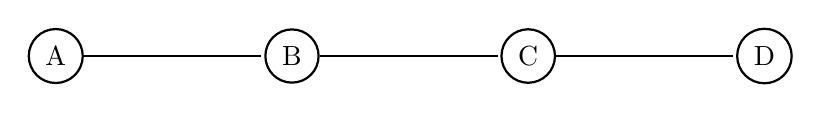
\begin{tikzpicture}[-,>=stealth',shorten >=1pt,auto,node distance=3cm, thick,main node/.style={circle,draw}, every loop/.style={}, scale=0.7]
            \node[main node] (A) {A};
            \node[main node] (B) [right of=A] {B};
            \node[main node] (C) [right of=B] {C};
            \node[main node] (D) [right of=C] {D};
            \path[every node/.style={font=\sffamily\small}]
            (A) edge node {} (B)
            (B) edge node {} (C)
            (C) edge node {} (D);
        \end{tikzpicture}}
        \end{center}

          \item \textbf{Bus Network}: All nodes are connected to a common medium along this medium. 

        \item \textbf{Star Network}: all nodes are connected to a special central node.
          \begin{center}
          \resizebox{3cm}{3cm}{%
          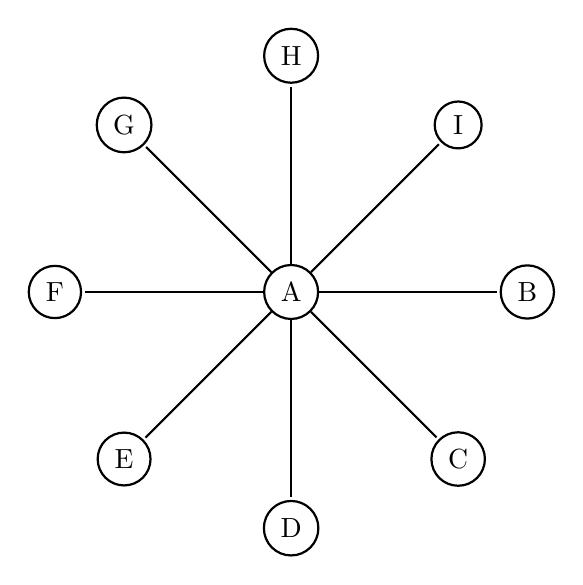
\begin{tikzpicture}[-,>=stealth',shorten >=1pt,auto,node distance=3cm, thick,main node/.style={circle,draw}, every loop/.style={}]
              \node[main node] (A) {A};
              \node[main node] (B) [right of=A] {B};
              \node[main node] (C) [below right of=A] {C};
              \node[main node] (D) [below of=A] {D};
              \node[main node] (E) [below left of=A] {E};
              \node[main node] (F) [left of=A] {F};
              \node[main node] (G) [above left of=A] {G};
              \node[main node] (H) [above of=A] {H};
              \node[main node] (I) [above right of=A] {I};
              \path[every node/.style={font=\sffamily\small}]
              (A) edge node {} (B)
              (A) edge node {} (C)
              (A) edge node {} (D)
              (A) edge node {} (E)
              (A) edge node {} (F)
              (A) edge node {} (G)
              (A) edge node {} (H)
              (A) edge node {} (I);
          \end{tikzpicture}}
          \end{center}

        \item \textbf{Ring Network}: Each node is connected to its left and right neighbour node, such that all nodes are connected and that each node can reach each other node by traversing nodes left- or rightwards.
          \begin{center}
          \resizebox{3cm}{3cm}{%
          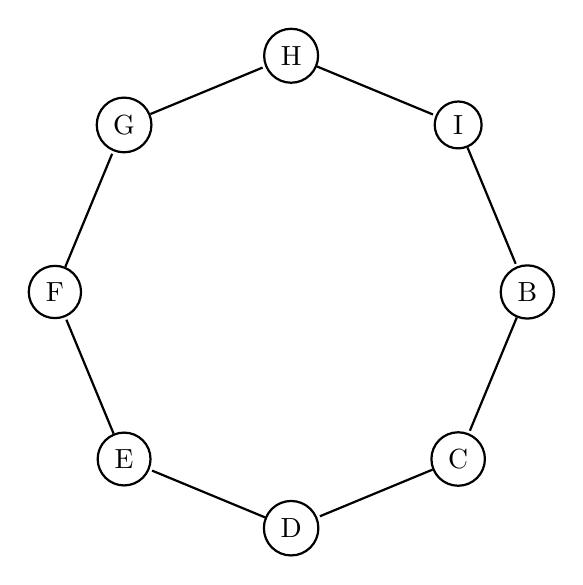
\begin{tikzpicture}[-,>=stealth',shorten >=1pt,auto,node distance=3cm, thick,main node/.style={circle,draw}, every loop/.style={}]
              \node[main node] (A) {A};
              \draw[white, fill=white] (-1,-1) rectangle (1,1);
              \node[main node] (B) [right of=A] {B};
              \node[main node] (C) [below right of=A] {C};
              \node[main node] (D) [below of=A] {D};
              \node[main node] (E) [below left of=A] {E};
              \node[main node] (F) [left of=A] {F};
              \node[main node] (G) [above left of=A] {G};
              \node[main node] (H) [above of=A] {H};
              \node[main node] (I) [above right of=A] {I};
              \path[every node/.style={font=\sffamily\small}]
              (B) edge node {} (C)
              (C) edge node {} (D)
              (D) edge node {} (E)
              (E) edge node {} (F)
              (F) edge node {} (G)
              (G) edge node {} (H)
              (H) edge node {} (I)
              (I) edge node {} (B);
          \end{tikzpicture}}
          \end{center}

        \item \textbf{Mesh Network}: each node is connected to an arbitrary number of neighbours in such a way that there is at least one traversal from any node to any other. 
          \begin{center}
          \resizebox{3.5cm}{3cm}{%
          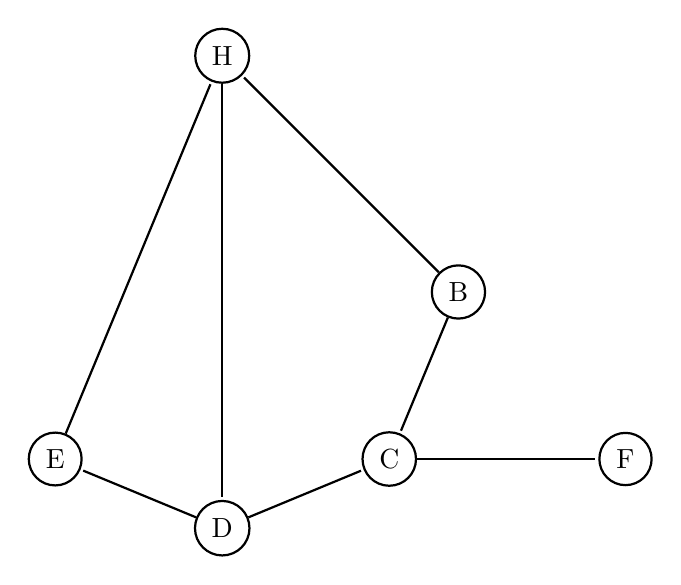
\begin{tikzpicture}[-,>=stealth',shorten >=1pt,auto,node distance=3cm, thick,main node/.style={circle,draw}, every loop/.style={}]
              \node[main node] (A) {A};
              \draw[white, fill=white] (-1,-1) rectangle (1,1);
              \node[main node] (B) [right of=A] {B};
              \node[main node] (C) [below right of=A] {C};
              \node[main node] (D) [below of=A] {D};
              \node[main node] (E) [below left of=A] {E};
              \node[main node] (H) [above of=A] {H};
              \node[main node] (F) [right of=C] {F};
              \path[every node/.style={font=\sffamily\small}]
              (B) edge node {} (C)
              (B) edge node {} (H)
              (D) edge node {} (C)
              (D) edge node {} (E)
              (C) edge node {} (F)
              (E) edge node {} (H)
              (H) edge node {} (D);
          \end{tikzpicture}}
          \end{center}

        \item \textbf{Fully Connected Network}: each node is connected to every other node in the network.
          \begin{center}
          \resizebox{3cm}{3cm}{%
          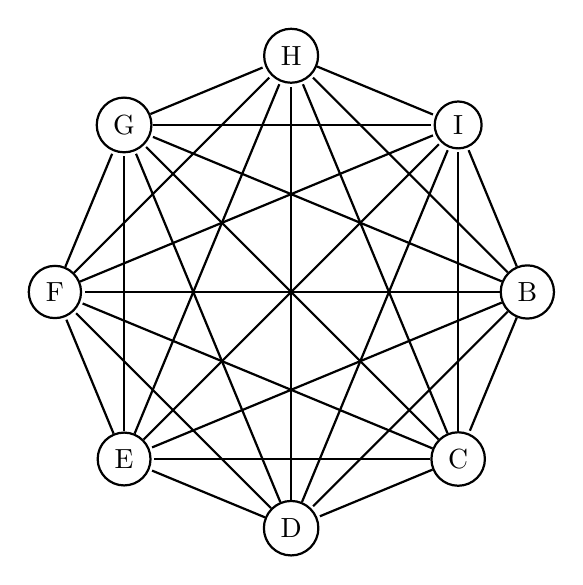
\begin{tikzpicture}[-,>=stealth',shorten >=1pt,auto,node distance=3cm, thick,main node/.style={circle,draw}, every loop/.style={}]
              \node[main node] (A) {A};
              \draw[white, fill=white] (-1,-1) rectangle (1,1);
              \node[main node] (B) [right of=A] {B};
              \node[main node] (C) [below right of=A] {C};
              \node[main node] (D) [below of=A] {D};
              \node[main node] (E) [below left of=A] {E};
              \node[main node] (F) [left of=A] {F};
              \node[main node] (G) [above left of=A] {G};
              \node[main node] (H) [above of=A] {H};
              \node[main node] (I) [above right of=A] {I};
              \path[every node/.style={font=\sffamily\small}]
              (B) edge node {} (C)
              (B) edge node {} (D)
              (B) edge node {} (E)
              (B) edge node {} (F)
              (B) edge node {} (G)
              (B) edge node {} (H)
              (B) edge node {} (I)
              (C) edge node {} (D)
              (C) edge node {} (E)
              (C) edge node {} (F)
              (C) edge node {} (G)
              (C) edge node {} (H)
              (C) edge node {} (I)
              (D) edge node {} (E)
              (D) edge node {} (F)
              (D) edge node {} (G)
              (D) edge node {} (H)
              (D) edge node {} (I)
              (E) edge node {} (F)
              (E) edge node {} (G)
              (E) edge node {} (H)
              (E) edge node {} (I)
              (F) edge node {} (G)
              (F) edge node {} (H)
              (F) edge node {} (I)
              (G) edge node {} (H)
              (G) edge node {} (I)
              (H) edge node {} (I);
          \end{tikzpicture}}
          \end{center}

        \item \textbf{Tree Network}: nodes are arranged hierarchically.
          \begin{center}
          \resizebox{5cm}{3cm}{%
          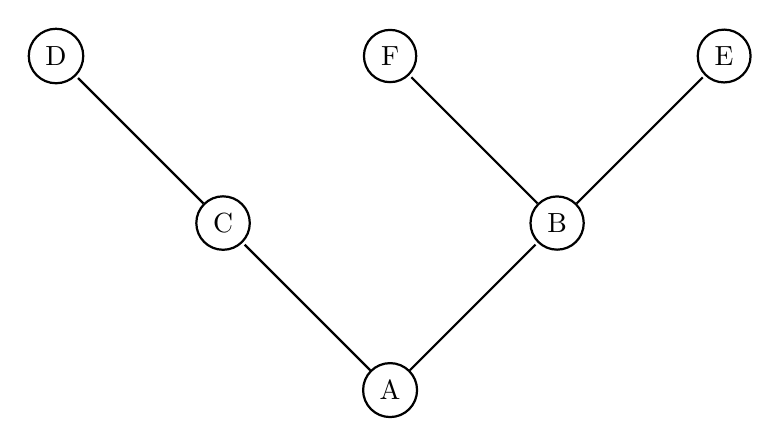
\begin{tikzpicture}[-,>=stealth',shorten >=1pt,auto,node distance=3cm, thick,main node/.style={circle,draw}, every loop/.style={}]
              \node[main node] (A) {A};
              \node[main node] (B) [above right of=A] {B};
              \node[main node] (C) [above left of=A] {C};
              \node[main node] (D) [above left of=C] {D};
              \node[main node] (E) [above right of=B] {E};
              \node[main node] (F) [above left of=B] {F};
              \path[every node/.style={font=\sffamily\small}]
              (A) edge node {} (B)
              (A) edge node {} (C)
              (B) edge node {} (F)
              (B) edge node {} (E)
              (C) edge node {} (D);
          \end{tikzpicture}}
          \end{center}
      \end{enumerate} 
    \end{example}

    Notice how many of these networks have \textbf{redundancy}: having multiple ways to get from one node to another. That is, when a network path is no longer available, data is still able to reach its destination through another path. Usually, we would like to avoid a \textbf{single point of failure} and construct a \textbf{fault-tolerant} system that can experience failure in its components but still continue operating properly. However, building more connections may be expensive. 

    Because there are multiple paths that a piece of data takes to get from point X to point Y, \textit{routing strategies} are implemented in order to determine the most optimal path. Now in order for network nodes to communicate with each other, they should have some sort of universal method of communicating with each other. 

    \begin{definition}[Communication Protocol]
      A \textbf{communication protocol} is a system of rules that allow multiple entities of a communications to transmit information via any kind variation of a physical quantity. The protocol defines the rules, syntax, semantics and synchronization of communication and possible error recovery methods. A protocol can have many jobs, such as: 
      
      \begin{enumerate} 
        \item Determining how nodes will communicate with each other . 
        \item Making sure that these modes of communication is compatible with hardware .
        \item Implementing security protocols such as encryption schemes. 
      \end{enumerate}
    \end{definition}

    Computers can connect through \textbf{physical} (e.g. cables) or \textbf{wireless} connections. 

    \begin{enumerate}
      \item The \textbf{CAT5 cable} is a \textit{twisted pair (copper) cable} that's designed for use in computer networks. It consists of four twisted pairs of copper wires. These twisted pair cables send data through a network by transmitting pulses of electricity that represent binary data. The information transmission follow the \textbf{Ethernet} standards, which is why twisted pair cables are commonly known as Ethernet cables. Use for both LANs and WANs. They can carry up to 1 Gbps across hundreds of feet, but are susceptible to interference. 

      \item \textbf{Fiber-optic cables} carry light instead of electricity in a fiber coated with plastic layers. The pulses of light represent binary data and also follow the Ethernet standards. They are also capable of transmitting much more data per second that copper cables, and they have the advantage of low transmission loss and immunity to electrical interference. Often used to connect networks across oceans so that data can travel quickly around the world. They can carry up to 26 Tbps acorss 50 miles (but are expensive)

      \item A wireless card inside a computer turns binary data into \textbf{radio waves} and transmits them through the air. However, they do not travel very far (~100 ft in office buildings or up to 1000 ft in an open field). The waves are picked up by a \textit{wireless access point} which converts them from radio waves back into binary data. These access points would be connected to the rest of the network using physical wiring. They can carry up to 1.3 Gbps. 

      \item \textbf{Infrared signals} and \textbf{microwaves} are sometimes used. 
    \end{enumerate}


    In order for the computers to send data into binary, they must convert this data into binary and send them as streams of 1s and 0s in a process called \textbf{line coding}. Furthermore, computers can raise efficiency of each wire by sending changing electric currents through a single wire. For example, rather than using three wires to encode $\texttt{101}$ as 

    \begin{center}
      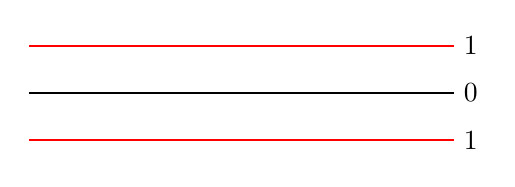
\begin{tikzpicture}[scale=0.6]
        \draw[thick, red] (0,1)--(9,1);
        \draw[thick] (0,0)--(9,0);
        \draw[thick, red] (0,-1)--(9,-1);
        \node[right] at (9,1) {1};
        \node[right] at (9,0) {0}; 
        \node[right] at (9,-1) {1};
      \end{tikzpicture}
    \end{center}

    they send it through a single wire with intervals of $\frac{1}{3}$ seconds

    \begin{center}
      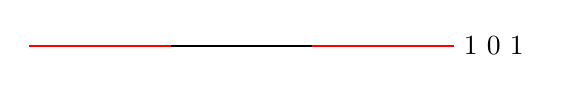
\begin{tikzpicture}[scale=0.6]
        \draw[thick, red] (0,0)--(3,0);
        \draw[thick] (3,0)--(6,0);
        \draw[thick, red] (6,0)--(9,0);
        \node[right] at (9,0) {1 0 1};
      \end{tikzpicture}
    \end{center}

    or even better, at a rate of 1 megabit per second (interval of $0.000001$ seconds)

    \begin{center}
      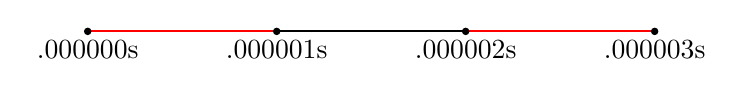
\begin{tikzpicture}[scale=0.8]
        \draw[thick, red] (0,0)--(3,0);
        \draw[thick] (3,0)--(6,0);
        \draw[thick, red] (6,0)--(9,0);
        \draw[fill] (0,0) circle (0.05);
        \draw[fill] (3,0) circle (0.05);
        \draw[fill] (6,0) circle (0.05);
        \draw[fill] (9,0) circle (0.05);
        \node[below] at (0,0) {.000000s};
        \node[below] at (3,0) {.000001s};
        \node[below] at (6,0) {.000002s};
        \node[below] at (9,0) {.000003s};
      \end{tikzpicture}
    \end{center}

    As long as two computers agree on the time period in which the electricity intervals are being sent, they can communicate much more efficiently. In an electrical connection (such as Ethernet), the signal would be a voltage or current. In an optical connection (such as a fiber-optic cable), the signal would be the intensity of light. 

    \begin{definition}
      There are many properties about line coding that are relevant, but ultimately the speed of a connection is a combination of the bandwidth and latency. 

      \begin{enumerate}
        \item The \textbf{bit rate} describes the data transfer rate of a connection. It measures the number of bit states that a channel can \textit{transmit} per unit time. It is measured in \textit{bits per second}. We can interpret it as the amount of water flowing through a pipe. 
        
        Bit rate is typically seen in terms of the actual data rate. But for most transmissions, the data represents part of a more complex protocol, which includes bits representing source address, destination address, error detection/correction codes, and other information. This data is called the \textbf{overhead}, while the actual data transferred is called the \textbf{payload}. At times, the overhead may be substantial (up to 20\% to 50\%). 

        \item The \textbf{throughput} is the number of bit states of usable information, that can be successfully \textit{received} over a channel per unit time. Without any channel noise, it is really just the payload. Note that this is an \textit{observed, dynamic parameter} with a fixed and variable loss. It is also known as \textbf{consumed bandwidth} and is measured in \textit{bits per second}. 
        
        \item The \textbf{bandwidth} describes the \textit{maximum} data transfer rate of a connection; that is, the maximum throughput of a communication. It is measured in \textit{bits per second}. We can interpret it as how thick the pipe is (i.e. how much water can flow through it at max). Note that this is different from the bandwidth used in signal processing. 
        
        Data often flows over multiple network connections, which means the connection with the smallest bandwidth (most likely your local connection) acts as a bottleneck. 
        
        \item The \textbf{latency}, or \textbf{ping-rate}, measures the round trip time between the sending of a data message to a computer and the receiving of that message, measured in \textit{milliseconds}. We can interpret it as the speed at which the water is flowing through a pipe. We can check latency by doing
        \begin{lstlisting}
          >>>ping www.google.com
          64 bytes: icmp_seq=0 ttl=115 time=37.868 ms
        \end{lstlisting}

        which outputs a latency time of 37.868ms (to get to $\texttt{www.google.com}$ and back) for sending a data packet of 64 bytes. Note that there is an intrinsic limiting factor to latency: the speed of light, which is approximately 1 foot per nanosecond. In addition to distance, another limiting factor is the congestion in the network and the type of connection. 
      \end{enumerate}
    \end{definition}

    \begin{example}
    Given two computers connected by a wire that is configured to transfer 1000 bits per second, the bit rate would be 1 Kbps. However, if the channel has noise and demands retransmission of 10 bits out of every 1000 of the original transmission, then the throughput would be 990 bps. 

    Furthermore, the Ethernet frame can have as many as 1542 bytes. Say that there are 1500 bytes of payload and an overhead of 42 bytes. Then, the \textbf{protocol efficiency} would would be 
    \[\frac{\text{payload}}{\text{frame size}} = \frac{1500}{1542} = 0.9727 = 97.3\%\]
    \end{example}

    Typically, the actual line rate is stepped up by a factor influenced by the overhead to achieve an actual target net data rate. In One Gigabit Ethernet, the actual line rate is 1.25 Gbits/s to achieve a net payload throughput of 1 Gbit/s. In a 10-Gbit/s Ethernet system, gross data rate equals 10.3125 Gbits/s to achieve a true data rate of 10 Gbits/s. The net data rate also is referred to as the throughput, or payload rate, of effective data rate.

  \subsection{History of the Internet}

    IETF, ICANN, IANA, ISPs.  

    \begin{example}[ARPANET]
      The ARPANET was the precursor to the Internet, the network where Internet technology was first tested out. It was started in 1969 with four computers connected to each other. 

        \begin{center}\resizebox{5cm}{3cm}{%
        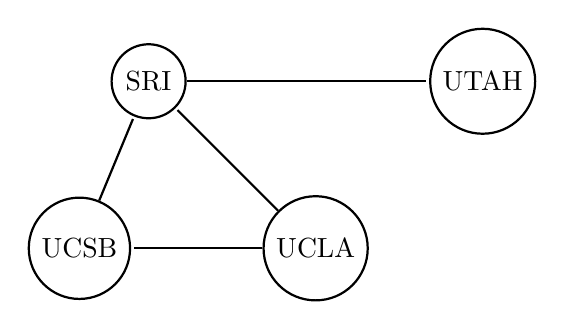
\begin{tikzpicture}[-,>=stealth',shorten >=1pt,auto,node distance=3cm, thick,main node/.style={circle,draw}, every loop/.style={}]
            \node[main node] (UCLA) {UCLA};
            \node[main node] (UCSB) [left of=UCLA] {UCSB};
            \node[main node] (SRI) [above left of=UCLA] {SRI};
            \node[main node] (UTAH) [above right of=UCLA] {UTAH};
            \path[every node/.style={font=\sffamily\small}]
            (UCLA) edge node {} (UCSB)
            (UCLA) edge node {} (SRI)
            (UCSB) edge node {} (SRI)
            (SRI) edge node {} (UTAH);
        \end{tikzpicture}}
        \end{center}

      For example, even if the path between SRI and UCSB is gone, the connections between SRI and UCSB is not lost (since IP packets can travel through UCLA's router). 
    \end{example}


    Now we can see an implementation of these networks in the internet. 

    \begin{definition}[Internet]
      The \textbf{Internet} is a global network of computing devices communicating with each other in some way, whether they're sending emails, downloading files, or sharing websites. The Internet is an \textbf{open network}, which means that any computing device can join as long as they follow the protocols. The internet is powered by many layers of protocols, and to create a global network of computing devices, we need: 

      \begin{enumerate}
        \item \textbf{Wires \& Wireless}: Physical connections between devices, plus protocols for converting electromagnetic signals into binary data. 
        \item \textbf{IP}: A protocol that uniquely identifies devices using IP addresses and provides a routing strategy to send data to a destination IP address. 
        \item \textbf{TCP/UDP}: Protocols that can transport packets of data from one device to another and check for errors along the way. 
        \item \textbf{TLS}: A secure protocol for sending encrypted data so that attackers can't view private information. 
        \item \textbf{HTTP \& DNS}: The protocols powering the World Wide Web
      \end{enumerate}        
    \end{definition}

    An \textbf{ISP (Internet Service Provider)} provides internet to its region. These ISPs are managed by certain continental autonomous systems (\textbf{AS}). The \textbf{Regional Internet Registry (RIR)} is divided into their regions: AFRNIC (Africa), ARIN (American), APNIC (Asia-Pacific), LACNIC (Latin America and Carribean), and RIPE NCC (European). 

    The main protocol suite used by the internet is \textbf{TCP/IP}, which is a collection of protocols that the internet uses. The bulk of this chapter will describe this protocol. 

    \begin{figure}[hbt!]
      \centering
      \includegraphics[scale=0.7]{img/tcp_ip_model.png}
      \caption{TCP/IP layering model. }
      \label{fig:tcp_ip_model}
    \end{figure}

  \subsection{Network Interfaces}

    Before we even start talking about IP addresses or protocols, we should mention that there are several interfaces from which computers can send and receive data. For example, if you are connected to both wired ethernet and WiFi, there are two paths, or interfaces, that data can travel. To see all your interfaces, use the \texttt{ip -c a} command. 

    \begin{lstlisting} 
      1: lo: <LOOPBACK,UP,LOWER_UP> mtu 65536 qdisc noqueue state UNKNOWN group default  
          link/loopback 00:00:00:00:00:00 brd 00:00:00:00:00:00
          inet 127.0.0.1/8 scope host lo
             valid_lft forever preferred_lft forever
          inet6 ::1/128 scope host noprefixroute 
             valid_lft forever preferred_lft forever
      2: wlan0: <BROADCAST,MULTICAST,UP,LOWER_UP> mtu 1500 qdisc noqueue state UP group 
          link/ether 64:bc:58:11:c0:24 brd ff:ff:ff:ff:ff:ff
          inet 10.197.221.245/16 brd 10.197.255.255 scope global dynamic noprefixroute 
             valid_lft 597085sec preferred_lft 597085sec
          inet6 fe80::b9e9:2f85:ded7:eaaf/64 scope link noprefixroute 
             valid_lft forever preferred_lft forever
    \end{lstlisting}

    The following lists out all the interfaces. We can see that we're connected to two interfaces, but there are a lot more. Usually, these interfaces also have a number following them that indexes different instances of the same type of interface. 

    \begin{enumerate} 
      \item \textbf{lo}: This is the loopback interface. 
      \item \textbf{wlan0}: For wireless connections 
      \item \textbf{tun}: When you are connected to VPN. 
      \item \textbf{en}: 
      \item \textbf{gif}: 
      \item \textbf{awd}: 
      \item \textbf{llw}: 
      \item \textbf{bridge}: 
      \item \textbf{utun}: 
    \end{enumerate}

    For each interface, there is a set of protocols that must be set for data to transfer. 

  \subsection{Addresses}

    Every computer needs some address that determines its unique identity. The version of TCP/IP that has been in widespread use is IPv4, which uses 4-byte IP addresses. A modernized version, IPv6, expands the IP address space to 16 bytes and incorporates several additional features, making it faster and easier to implement. 

    \begin{definition}[IP Address]
      The protocol describes the use of \textbf{IP addresses} to uniquely identify Internet-connected devices (for transmission of data). That is, when a computer sends a message to another computer, it must specify the recipient's IP address and also include its own IP address so that the second computer can reply. There are two versions of the Internet Protocol in use today: 
      \begin{enumerate}
          \item \textbf{IPv4}: The first version ever used on the Internet and having the form of 4 \textit{octets} split by periods in between. 

            \[[0-255].[0-255].[0-255].[0-255]\]

          Even though it presented in decimal, computers store them in binary 

            \[74.125.20.113 \iff 01001011.01111101.00010100.01110001\]

          IPv4 addresses can take $2^{32}$ values, but IPv6 was created for more space.

          \item \textbf{IPv6}: The newer standard (introduced in June 2012) is in the form 

            \[\text{FFFF:FFFF:FFFF:FFFF:FFFF:FFFF:FFFF:FFFF}\]

          with hexadecimal digits (total of ~$3.4 \times 10^{39}$ possible IPv6 values). 
      \end{enumerate}
    \end{definition}


    \begin{definition}[CIDR Notation]
      Sometimes, a set of IP addresses are specified using \textbf{CIDR notation}. An address of the form 

        \[145.201.67.4/16\]

      represents all addresses of form $145.201.\ast.\ast$. 
    \end{definition}

    Operating systems and network devices have supported IPv6 for a long time, and the motivation behind the deployment of IPv6 was due to the concern that devices were running out of IPv4 addresses. Asia ran out first in 2011, followed by every other continent ever since then. 

    But we've learned to make more efficient use of the IPv4 addresses that we have. For example, \textbf{Network Address Translation} (or \textbf{NAT}) lets entire networks of machines hide behind single IPv4 addresses. \textbf{Classless Inter-Domain Routing} (\textbf{CIDR}) subdivides networks and promotes efficient backbone routing as well. Ultimately, IPv6, with better security and engineering, is going to take over, but not for a while since it's not fundamentally different from IPv4 and the drawbacks of IPv4 haven't been bad enough to spark migration. 

    \begin{definition}[Hierarchy of IP Addresses] 
      The IP addresses are formatted in an \textit{hierarchical way}. The IPv4 address hierarchy is structured as such: The first few numbers (may or may not be divided by octets) could identify a \textbf{network} administered by an Internet Service Provider. The last numbers, which can also represent \textbf{subnetworks} (subnets), identifies a home computer on that network. 
    \end{definition}

    \begin{example}[University of Michigan]
      For example, if we represent the IP address 141.213.127.13 in binary (of 32 bits)

        \[10001101.11010101.01111111.00001101\]

      the first 16 bits could route to all of UMich, the next two bits could route to a specific UMich department, and the final 14 bits could route to individual computers. 
      \begin{center}
      \begin{tabular}{l|l|l}
          1000110111010101 & 01 & 11111100001101  \\
          \hline
          UMich Network & Medicine department & Lab computer 
      \end{tabular}
      \end{center}
      This hierarchy gives UMich the ability to differentiate between $2^2$ departments and $2^{14} = 16,384$ computers within each department. In general, the ability to create hierarchical levels at any point in the IP address allows for greater flexibility in the size of each level of the hierarchy. 
    \end{example}
    
    \begin{example}[Duke]
      Duke's IP addresses are of the form $153.3.\_.\_$, with the DUKE-INTERCHANGE ISP provider.  
    \end{example} 

    \begin{definition}[Hostname]
      IP addresses can be quite cumbersome to memorize, which is why they are often addressed with their \textbf{hostname}. Operating systems allow one or more hostnames to be associated with an IP address so that users can type \texttt{rfc-editor.org} rather than $4.31.198.49$. This mapping can be set up  in multiple days, e.g. with the \texttt{/etc/hosts} file or the LDAP database system to DNS the world-wide \textbf{Domain Name System}. 
    \end{definition}

    \subsubsection{LAN Addresses and NAT} 

      We've talked about how entire networks of machines can hide behind a single IPv4 address. Let's elaborate on this. In fact, your computer is not connected to the internet directly. It is actually in a \textbf{private network}, or a \textit{LAN network}, which uses a private IP address space (supported by both IPv4 and v6). Anything on the inside of your private network is not on the Internet; it is on your LAN, an entirely separate network, with its own address space. Anything on your LAN must have a unique (within the LAN) IP address to participate properly with your local network. Therefore, anyone else who has a LAN is also not part of the internet. So if you are only on your LAN network, how do you actually connect to the internet? 

      \begin{definition}[Router] 
        The \textbf{router} is a device that forms a connection between your LAN network and the internet. It has both a private local address, called a \textbf{gateway address}, and a public address. It is responsible for forwarding data between the local server computers and the internet. Therefore, to the outside world, all devices identify the network internet activity by the one public IP address assigned to the router. 

        The gateway address can be found with \texttt{ip route} and the public address, of course, can be found with the commands previously mentioned. 
      \end{definition}

      \begin{definition}[Modem]
        A \textbf{modem}, short for \textbf{modulator/demodulator} is a device that converts a signal from your computer to some kind of signal to talk to other computers. The main difference between the router and the modem is that 
        \begin{enumerate} 
           \item The router crates a network between the computers in your home and routes network traffic between them (through Ethernet cables or wireless connection). Your home router has one connection to the Internet and connections to your private local network. 

          \item The modem serves as a bridge between your local network and the Internet.  
        \end{enumerate}
      \end{definition}

      To access our IP address, we can do the following: 
      \begin{enumerate} 
        \item To access local ip address, we can either run the command \texttt{hostname -i}, \texttt{ip -c a}, or \texttt{ifconfig}.
          
        \item To access the public ip address, we can either google it or run \texttt{curl ifconfig.me}. Since this is public, any device connected to the same network/router should have the same IP address. 
      \end{enumerate}

      \begin{definition}[NAT]
        In order for LAN devices to connect to the Internet, their outgoing traffic has the source address changed to match that of the internet/WAN IP address of the router. The router keeps track of this, and makes sure any response traffic gets sent to the right internal machine. This is called \textbf{Network Address Translation (NAT)}. There are generally two types of NAT: 

        \begin{enumerate}
          \item \textbf{Basic, one-to-one NAT}: The simplest type of NAT provides a one-to-one translation of IP addresses. In this type of NAT, only the IP addresses, IP header checksum, and any higher-level checksums that include the IP address are changed. Basic NAT can be used to interconnect two IP networks that have incompatible addressing. 

          \item \textbf{One-to-many NAT}: The majority of network address translators map multiple private hosts to one publicly exposed IP address. In a typical configuration, a local network uses one of the designated private IP address subnets. A router in that network has a private address of that address pace. The router it also connected to the Internet with a \textit{public} address assigned by the ISP. As traffic passes from the local network to the Internet, the source address in each packet is translated on the fly from a private address to the public address. The router tracks basic data about each active connection (particularly the destination address and port). When a reply returns to the router, it uses the connection tracking data it stored during the outbound phase to determine the private address on the internal network to which to forward the reply. 
        \end{enumerate}
      \end{definition}

      \begin{definition}
        The IP addresses that are in the private network's space are usually divided up into 3 categories. But as of now, the categories don't mean anything. 

        \begin{enumerate}
          \item \textbf{Class A private range addresses}: 10.0.0.0 - 10.255.255.255 (16,777,216 IPs)
          \item \textbf{Class B private range addresses}: 172.16.0.0 – 172.31.255.255 (1,048,576 IPs)
          \item \textbf{Class C private range addresses}: 192.168.0.0 – 192.168.255.255 (65,536 IPs)
        \end{enumerate}

        Since the private IPv4 address space is relatively small, many private IPv4 networks unavoidably use the same address ranges. This can create a problem when merging such networks, as some addresses may be duplicated for multiple devices. In this case, networks or hosts must be renumbered, often a time-consuming task, or a network address translator must be placed between the networks to translate or masquerade one of the address ranges. 
      \end{definition}


    \subsubsection{Ports}

      IP addresses identify a machine's network interfaces, but they aren't specific enough to address individual processes or services, many of which might be actively using the network at once. TCP and UDP extend IP addresses with a concept known as a port, which is a 16-bit number that supplements an IP address to a particular communication channel. Valid ports range from $1$ to $65,535$. A port, combined with an IP address, results in a \textbf{socket address} that is used to establish a connection between a client and a server. 

      UNIX systems restrict programs from binding to port numbers under 1024 unless they are run as root or have an appropriate Linux capability. Anyone can communicate with a server running on a low port number; the restriction only applies to the program listening on the port.

    \subsubsection{Hardware (MAC) Addresses}

      The lowest level of addressing is the network hardware. Many devices are assigned a unique 6-byte hardware address at the time of manufacture. The first 3 bytes identify the manufacturer, and the last 3 bytes are a unique serial number that the manufacturer assigns. Sysadmins can sometimes identify the brand of machine that is trashing a network by looking up the 3-byte identifier in a table of vendor IDs. In theory, ethernet hardware addresses are permanently assigned and immutable, but many network interfaces let you override the hardware address and set one of your own choosing. 

  \subsection{TCP Packets and Encapsulation}

  \subsection{OSI and Internet Protocols}
  

  \subsection{HTTP and HTTPS} 

    HTTP stands for hypertext transfer protocol, implemented in Layer 7, which transfers data between your computer and the server over the internet through \textbf{clear text}. This may not be the most ideal way since any interceptors can read the transferred data. This isn't a problem for regular internet browsing, but if you are inputting sensitive data, then HTTP should not be used. This is why HTTPS (which stands for secure HTTP) was invented, which  is implemented in Layer 4 and encrypts the data being transferred, and every website where you input sensitive data should be using HTTPS (indicated by the \texttt{https://} prefix in the URL and a padlock symbol for modern browsers). Due to the extra security measures, HTTPS is less lightweight than HTTP, and its respective default ports are HTTP (80) and HTTPS (443).  

    A natural question to ask would be: which encryption scheme does HTTPS use? Both Secure Sockets Layer (SSL) and Transport Layer Security (TLS) is used in the modern web. 

    SSL certificate. 

    
  \subsection{UDP and TCP}

    TCP handshake can be seen with curl. 


\section{Driver and Hardware Configuration}

  \subsection{Audio Drivers} 


  \subsection{Bluetooth}
    Blueman. 

  \subsection{Synaptics}


  \subsection{Video Drivers}


  \subsection{Monitor}


  \subsection{Nvidia GPU Drivers} 

  \subsection{Camera Settings}

    I have a Nexigo N60 camera. The company provides webcam drivers for Windows and Mac, but not Linux, so I use the \textbf{v4l2} (video4linux) package. To list all camera devices, type 
    \begin{lstlisting}
    (base) mbahng@xps15:~$ v4l2-ctl --list-devices
    Integrated_Webcam_HD: Integrate (usb-0000:00:14.0-11):
      /dev/video2
      /dev/video3
      /dev/video4
      /dev/video5
      /dev/media1
      /dev/media2

    NexiGo N60 FHD Webcam Audio: Ne (usb-0000:00:14.0-3.1):
      /dev/video0
      /dev/video1
      /dev/media0
    \end{lstlisting}
    You should identify which folder path corresponds to which video camera. 
    \begin{lstlisting}
    (base) mbahng@xps15:~$ v4l2-ctl --list-ctrls --device /dev/video0

    User Controls

                         brightness 0x00980900 (int)    : min=0 max=255 step=1 default=128 value=20
                           contrast 0x00980901 (int)    : min=0 max=255 step=1 default=128 value=128
                         saturation 0x00980902 (int)    : min=0 max=255 step=1 default=128 value=128
            white_balance_automatic 0x0098090c (bool)   : default=1 value=1
                               gain 0x00980913 (int)    : min=0 max=100 step=1 default=5 value=5
               power_line_frequency 0x00980918 (menu)   : min=0 max=2 default=1 value=2 (60 Hz)
          white_balance_temperature 0x0098091a (int)    : min=2600 max=6500 step=1 default=4650 value=4650 flags=inactive
                          sharpness 0x0098091b (int)    : min=0 max=255 step=1 default=128 value=128

    Camera Controls

                      auto_exposure 0x009a0901 (menu)   : min=0 max=3 default=0 value=1 (Manual Mode)
             exposure_time_absolute 0x009a0902 (int)    : min=0 max=6500 step=1 default=100 value=100
                       pan_absolute 0x009a0908 (int)    : min=-36000 max=36000 step=3600 default=0 value=0
                      tilt_absolute 0x009a0909 (int)    : min=-36000 max=36000 step=3600 default=0 value=0
         focus_automatic_continuous 0x009a090c (bool)   : default=0 value=0
                      zoom_absolute 0x009a090d (int)    : min=10 max=20 step=1 default=10 value=10

    \end{lstlisting}
    Then to set the controls, you write 
    \begin{lstlisting}
    v4l2-ctl -d /dev/video0 --set-ctrl=auto_exposure=1
    \end{lstlisting}

\end{document}

